\documentclass[a4paper,12pt,twoside]{article}
\usepackage[left=1in,right=1in,top=1in,bottom=1in]{geometry}

\usepackage{xeCJK}
\setCJKmainfont{Songti TC}
\setCJKfamilyfont{kai}{Songti TC}
\newcommand{\kai}{\CJKfamily{kai}} % 用 \kai{使用楷書}

\usepackage{lmodern}
\usepackage{titling}
\usepackage{titlesec}
\usepackage{graphicx}
\usepackage{float}
\usepackage{amsmath, amsthm, amssymb, amsfonts, mathrsfs}
\usepackage{upgreek} % 直立的希臘字母

\usepackage[shortlabels]{enumitem}
\usepackage{setspace}
\renewcommand{\baselinestretch}{1.5}
\usepackage[colorlinks]{hyperref}
\usepackage{fancyvrb}
\usepackage{fancyhdr}
\usepackage{multicol}
\usepackage{caption}
\usepackage{listings}
\usepackage{bm}
\usepackage{bbm} % for \mathbbm{1} (indicator function)
\usepackage{centernot}
\usepackage{mdframed}
\usepackage{tikz}
\usetikzlibrary{patterns, arrows.meta, positioning}
\usepackage[nameinlink, capitalise]{cleveref}
\usepackage{diagbox}
\usepackage{booktabs}
\usepackage{multirow,array}
\usepackage{tabularx}
\usepackage{mathtools}
\usepackage{indentfirst} % 首段 indent
\setlength{\parindent}{2em}
\usepackage{cancel} % 數學式子畫線槓掉
\newcommand\mcancel[2][red]{\setbox0=\hbox{$#2$}%
\rlap{\raisebox{.45\ht0}{\textcolor{#1}{\rule{\wd0}{1pt}}}}#2}
\usepackage{datetime2}

\AtBeginDocument{%
 \setlength{\abovedisplayskip}{6pt}
 \setlength{\belowdisplayskip}{6pt}
 \setlength{\abovedisplayshortskip}{4pt}
 \setlength{\belowdisplayshortskip}{4pt}
}

\definecolor{codegreen}{rgb}{0,0.6,0}
\definecolor{codegray}{rgb}{0.5,0.5,0.5}
\definecolor{codepurple}{rgb}{0.58,0,0.82}
\definecolor{backcolour}{rgb}{0.95,0.95,0.92}

\lstdefinestyle{mystyle}{
 backgroundcolor=\color{backcolour},
 commentstyle=\color{codegreen},
 keywordstyle=\color{magenta},
 numberstyle=\tiny\color{codegray},
 stringstyle=\color{codepurple},
 basicstyle=\ttfamily\footnotesize,
 breakatwhitespace=false,
 breaklines=true,
 captionpos=b,
 keepspaces=true,
 numbers=left,
 numbersep=5pt,
 showspaces=false,
 showstringspaces=false,
 showtabs=false,
 tabsize=2
}
\lstset{style=mystyle}

\hypersetup{citecolor=blue, linkcolor=blue, urlcolor=blue}

\DeclareMathOperator{\supp}{supp}
\DeclareMathOperator{\skewness}{Skewness}
\DeclareMathOperator{\DU}{D-U}
\DeclareMathOperator{\CU}{C-U}
\DeclareMathOperator{\Geo}{Geo}
\DeclareMathOperator{\Pois}{Pois}
\DeclareMathOperator{\Gam}{Gam}
\DeclareMathOperator{\LN}{LogN}
\DeclareMathOperator{\cov}{Cov}
\DeclareMathOperator*{\argmax}{arg\,max}
\DeclareMathOperator*{\argmin}{arg\,min}
\DeclareMathOperator{\re}{Re}
\DeclareMathOperator{\im}{Im}

\newcommand{\N}{\mathbb{N}}
\newcommand{\Z}{\mathbb{Z}}
\newcommand{\Q}{\mathbb{Q}}
\newcommand{\R}{\mathbb{R}}
\newcommand{\C}{\mathbb{C}}
\newcommand{\G}{\mathcal{G}}
\newcommand{\mP}{\mathbb{P}}
\newcommand{\F}{\mathcal{F}}
\newcommand{\B}{\mathcal{B}}
\newcommand{\1}{\mathbbm{1}}
\newcommand{\Poi}{\text{Poi}}
\newcommand{\Var}{\text{Var}}
\newcommand{\as}{\text{a.s.}}
\newcommand{\vect}[1]{\boldsymbol{\mathbf{#1}}}
\newcommand{\paren}[1]{\left({#1}\right)}
\newcommand{\brk}[1]{\left[{#1}\right]}
\newcommand{\curl}[1]{\left\{{#1}\right\}}
\renewcommand{\lambda}{\lambdaup}

\theoremstyle{definition} % 定理環境 style 改用正體
\newtheorem{theorem}{定理}
\newtheorem{definition}{定義}
\newtheorem*{definition*}{定義}
\newtheorem{example}{例子}
\newtheorem{exercise}{練習}
\newtheorem{corollary}{推論}
\newtheorem{property}{性質}
\newtheorem{prop}{命題}
\newtheorem{lemma}{引理}
\newtheorem{problem}{問題}
\newtheorem*{remark}{註}

\renewcommand{\figurename}{圖}
\renewcommand{\tablename}{表}

\DeclareMathOperator{\var}{Var}
\DeclareMathOperator{\corr}{corr}
\DeclareMathOperator{\rank}{rank}
\DeclareMathOperator{\MSE}{MSE}
\DeclareMathOperator{\SSE}{SSE}
\DeclareMathOperator{\SST}{SST}
\DeclareMathOperator{\SSR}{SSR}
\DeclareMathOperator{\sgn}{sign}
\DeclareMathOperator{\alt}{Alt}
\DeclareMathOperator{\adj}{adj}
\DeclareMathOperator{\curlOp}{curl}
\DeclareMathOperator{\spn}{span}
\DeclareMathOperator{\sse}{SSE}
\DeclareMathOperator{\tr}{tr}

\newcommand{\ep}{\varepsilon}
\newcommand{\p}{\partial}
\newcommand{\abs}[1]{\left|#1\right|}
\newcommand\norm[1]{\left\lVert#1\right\rVert}
\newcommand{\innerprod}[1]{\langle#1\rangle}
\newcommand{\ds}{\displaystyle}
\newcommand{\blank}{\rule[-1mm]{1.5cm}{0.1mm}}
\newcommand{\dint}{\displaystyle\int}
\renewcommand{\bar}{\overline}

\newtheoremstyle{remark}{}{}{}{}{\bfseries\sffamily}{.}{.5em}{#1}
\theoremstyle{remark}

\newtheorem*{remark*}{\textit{Remark}}
\newtheorem*{solution*}{解}

\AtEndEnvironment{solution*}{\hfill$\square$}
\newtheorem*{hint*}{Hint}


\newcommand{\redtext}[1]{{\color{red} #1}}
\newcommand{\bluetext}[1]{{\color{blue} #1}}

\fancypagestyle{firstpage}{
  \fancyhf{}
  \fancyhead[R]{\small《高中數學實驗教材》第 4 冊（自然組）}
  \fancyhead[L]{\small 第 1 章\quad 座標變換與線性映射}
  \fancyfoot[C]{\thepage}
}

\pagestyle{fancy}
\setlength{\headheight}{14pt}
\renewcommand{\headrulewidth}{0.5pt}
\renewcommand{\footrulewidth}{0pt}
\fancyhead{}
\fancyhead[LE]{\small 《高中數學實驗教材》第四冊（自然組）}
\fancyhead[RO]{\small 第一章\quad 座標變換與線性映射}
\fancyfoot[C]{\thepage}

\title{\LARGE\textbf{《高中數學實驗教材》第四冊（自然組）}\\[0.5em] \Large\textbf{第一章\quad 座標變換與線性映射}}
\author{\textbf{高中數學實驗教材編輯小組}\quad 編著}
\date{民國六十五年（1976）三版}

\begin{document}

\maketitle
\thispagestyle{firstpage}

% ==========================================
% 掃描檔勘誤、文字校訂與疑難處說明（依規則整理於目錄之前）
% ==========================================
\section*{【說明】第一章掃描檔勘誤、疑難處與文義校訂表}
\addcontentsline{toc}{section}{【說明】第一章掃描檔勘誤、疑難處與文義校訂表}
\label{sec:errata_notes_b4_ch1}

本章依據 1976 年三版《高中數學實驗教材 第四冊（自然組）》（高二下）第一章「座標變換與線性映射」掃描原件完整轉錄為 \LaTeX{} 格式。為忠實反映教材原始內容並兼顧排版品質與嚴謹性，依作業規範將掃描檔中出現之印刷訛誤、符號缺漏、字模損毀、歷史印記雜訊及文義疑難處詳細考證彙整於下表。讀者可點擊表格中之章節連結直接跳至正文對應位置：

\begin{table}[H]
\centering
\small
\renewcommand{\arraystretch}{1.35}
\begin{tabularx}{\textwidth}{|p{3.2cm}|p{3.8cm}|X|}
\hline
\textbf{章節位置} & \textbf{掃描檔原始現象 / 誤植} & \textbf{考證說明與校訂處理} \\ \hline

\hyperref[note:b4-ch1-p2-bubiang]{§ I-1 頁 2 剛性運動不變性} & 
「長度在剛性運動（§ I-4）下不赞」 & 
原書印作「不赞」，顯為「不變」之鉛字印刷訛字。正文予以校訂並加註備查。 \\ \hline

\hyperref[note:b4-ch1-p2-bubiangliang]{§ I-1 頁 2 不變量異體字模} & 
「若對長度這一不孌量作深一層的分析」 & 
原書印作「不孌量」，為「不變量」之字模異寫。正文校訂為「不變量」並備註。 \\ \hline

\hyperref[note:b4-ch1-p2-pingyi]{§ I-1 頁 2 剛性運動組成成分} & 
「剛性運動不外是干移，旋轉，鏡射或其複合」 & 
原書印作「干移」，實為「平移」之排版訛字。正文予以校訂並備註。 \\ \hline

\hyperref[note:b4-ch1-p3-zhixian]{§ I-1 頁 3 例 1 鐵路線形描述} & 
「縱貫鐵路為一南北向之真線 $L$」 & 
原書印作「真線」，實為「直線」之排版訛字。正文予以校訂並備註。 \\ \hline

\hyperref[note:b4-ch1-p7-fig2-1]{§ I-2 頁 7 節段插圖編號體例} & 
插圖標為「圖 2-1」、「圖 2-2」等 & 
原書圖號採以小節號「§ I-2」作為首碼之歷史編排體例。正文忠實保留原刊編號並加註說明。 \\ \hline

\hyperref[note:b4-ch1-p16-lorentz]{§ I-2 頁 16 相對論選授標記} & 
「**【論例 2】（相對性原理）」 & 
對應原書目次「注意 1」提及「節段前加『**』指示可以不講授的部份」。正文忠實再現並加註說明。 \\ \hline

\hyperref[note:b4-ch1-p57-appendix-note]{§ I-5 頁 57 章末附註現代術語} & 
嵌射（injective）、蓋射（surjective）、對射（bijective） & 
轉錄時忠實保留 1970 年代現代數學結構之原有名詞與定義，同時附錄其現代通稱（單射、全射、雙射）。 \\ \hline

\end{tabularx}
\caption{第一章掃描檔勘誤、疑難處與文義校訂表}
\label{tab:errata_b4_ch1}
\end{table}

\vspace{1em}
\hrule
\vspace{1em}

\tableofcontents
\newpage

% =========================================================================
% 《高中數學實驗教材》第四冊（自然組）
% 第一章 座標變換與線性映射
% =========================================================================

\section{座標變換與線性映射}
\label{sec:b4-ch1}

\begin{center}
\begin{minipage}{0.75\textwidth}
\begin{itemize}[leftmargin=2em, itemsep=0.3em]
  \item[§ I-1] \textbf{直線的座標化及其上的座標變換}
  \item[§ I-2] \textbf{平面上的座標變換}
  \begin{itemize}[leftmargin=2em, itemsep=0.2em]
    \item[甲、] 平移
    \item[$\ddagger$ 乙、] 一般性的座標變換
  \end{itemize}
  \item[§ I-3] \textbf{平面上的線性映射}
  \begin{itemize}[leftmargin=2em, itemsep=0.2em]
    \item[甲、] 線性映射的意義
    \item[乙、] 線性映射的基本性質
    \item[丙、] 線性映射的矩陣表示
    \item[丁、] 線性映射的聯立式
  \end{itemize}
  \item[§ I-4] \textbf{剛性運動與正交線性映射}
  \begin{itemize}[leftmargin=2em, itemsep=0.2em]
    \item[甲、] 剛性運動
    \item[乙、] 正交線性映射
    \item[丙、] 旋轉與鏡射
    \item[丁、] 總結
  \end{itemize}
  \item[§ I-5] \textbf{正交座標變換}
\end{itemize}
\end{minipage}
\end{center}

\begin{center}
$* \qquad * \qquad * \qquad * \qquad *$
\end{center}

關於座標變換，我們其實在第三冊座標幾何一章的開頭便已談到一些，那裏我們舉例考慮過對於一個點，若已知其相關於某一正交座標系的座標，如何繪圖求得這點相關於另一一般座標系的座標．

本章我們將利用已熟習的向量及聯立方程式的求解，來處理座標變換的一般問題．同時我們強調一個座標系就相當於一個觀測系統這樣的觀點．

在種種事物中，藉用討論不變性或不變量的立場來看問題，常可了解問題的本質，例如在日常空間中，長度這一概念不因取另一正交座標系而作任何改變，換句話說，長度在剛性運動（§ I-4）下不變\phantomsection\label{note:b4-ch1-p2-bubiang}\footnote{【原書註記/校訂】：原書印作「不赞」，顯為「不變」之鉛字印刷訛字，茲予校訂．}，稱它為剛性運動下的一個不變量．若對長度這一不變量\phantomsection\label{note:b4-ch1-p2-bubiangliang}\footnote{【原書註記/校訂】：原書印作「不孌量」，為「不變量」之字模異寫．}作深一層的分析，發覺很多空間或平面的幾何性質都源自於它，這話實際上就相當於「向量的內積對空間或平面的構造起了決定性的作用」這一事實．（注意長度與向量內積相互決定！〔§ I-4 甲段本文及習題 I-4 第 4 題〕）

在這層意義下要了解不變量就相當於要了解這運動本身，在歐幾里得空間或平面裏，最重要的就是剛性運動，在 § I-4 中我們證明了剛性運動不外是平移\phantomsection\label{note:b4-ch1-p2-pingyi}\footnote{【原書註記/校訂】：原書印作「干移」，顯為「平移」之排版訛字，茲予校訂．}，旋轉，鏡射或其複合．（在 § I-2 結尾我們以嘗試性的姿態舉了相對性原理，作為論例，說明當兩個座標系間有很大的相對速度時，甚至連「長度」這一概念也不再是不變量．但在我們日常實驗室外所接觸到物體的運動因不牽涉極高的相對速度，古典力學的看法仍應無條件地被接受且研習．）

% =========================================================================
% § I-1 直線的座標化及其上的座標變換
% =========================================================================
\subsection{直線的座標化及其上的座標變換}
\label{sec:b4-1-1}

給定一條直線 $L$，取其上一點 $O$，再取一個不同於 $O$ 的點 $E$，設 $\tilde{\mathbf{e}} = \vec{OE}$，則對 $L$ 上任意點 $P$，$\vec{OP}$ 均為 $\tilde{\mathbf{e}}$（或正或負）的實倍數，亦卽存在一個實數 $x$，使得
\begin{equation}
\vec{OP} = x \tilde{\mathbf{e}} \label{eq:b4-1-1-1}
\end{equation}
由於 $L$ 上 $P$ 點與實數 $x$ 的對應是一對一的，故 $L$ 上的點，可乾脆以其對應的實數來描寫，基於此，我們稱 $(O; \tilde{\mathbf{e}})$ 為 $L$ 上的一個座標系，有時簡記以 $S$，寫成 $S \equiv (O; \tilde{\mathbf{e}})$，$L$ 上任意點 $P$ 根據 \eqref{eq:b4-1-1-1} 所得的相應的 $x$ 稱為 $P$ 點相關於 $S$ 的座標，簡記為 $S$---座標，其中 $O$ 點稱為這座標系 $S$ 的基準點〔註〕，$\tilde{\mathbf{e}}$ 稱為 $S$ 的基底，$\tilde{\mathbf{e}}$ 也稱為 $L$ 的一個基底．

\begin{figure}[H]
\centering
\begin{tikzpicture}[scale=1.1]
  % Top line: x = 1.5
  \draw[thick, -Stealth] (-1, 1.2) -- (6.5, 1.2) node[above left] {$L$};
  \filldraw (1, 1.2) circle (1.5pt) node[below] {$O$};
  \filldraw (3, 1.2) circle (1.5pt) node[below] {$E$};
  \filldraw (4, 1.2) circle (1.5pt) node[below] {$P$};
  \draw[very thick, -Stealth, blue] (1, 1.2) -- (3, 1.2) node[midway, above] {$\tilde{\mathbf{e}}$};
  \node at (2.5, 0.6) {\small （此圖 $P$ 點對應於實數 $1.5$）};

  % Bottom line: x = -0.6
  \draw[thick, -Stealth] (-2.5, -0.6) -- (5, -0.6) node[above left] {$L$};
  \filldraw (1, -0.6) circle (1.5pt) node[below] {$O$};
  \filldraw (3, -0.6) circle (1.5pt) node[below] {$E$};
  \filldraw (-0.2, -0.6) circle (1.5pt) node[below] {$P$};
  \draw[very thick, -Stealth, blue] (1, -0.6) -- (3, -0.6) node[midway, above] {$\tilde{\mathbf{e}}$};
  \node at (1.5, -1.2) {\small （此圖 $P$ 點對應於實數 $-0.6$）};
\end{tikzpicture}
\caption{直線座標系}
\label{fig:b4-1-1}
\end{figure}

這樣的一種座標化實際上可以看成是一個觀測者所選定的一種觀測系統．

先考慮下面的一個實例：

\begin{example}[例 1]
設一火車在縱貫鐵路上行駛（姑且假定縱貫鐵路為一南北向之直線\phantomsection\label{note:b4-ch1-p3-zhixian}\footnote{【原書註記/校訂】：原書印作「南北向之真線」，「真線」顯為「直線」之排版訛字，茲予校訂．} $L$）有甲乙兩名觀測員皆想描述這火車正午時的位置 $P$，甲從臺北算起，測得 $P$ 點在臺北站南下 $338.93$ 公里處．乙觀測者想從臺中站，以英里（哩）往南計算測 $P$ 點應在何處？
\end{example}

\begin{figure}[H]
\centering
\begin{tikzpicture}[scale=0.95]
  % Rail line
  \draw[thick, -Stealth] (-0.5, 0) -- (12.5, 0) node[right] {南};
  % Stations
  \filldraw (0.5, 0) circle (2pt) node[below=3pt] {$O$} node[above=3pt] {臺北};
  \filldraw (4.5, 0) circle (2pt) node[below=3pt] {$O'$} node[above=3pt] {臺中};
  \filldraw (8.5, 0) circle (2pt) node[below=3pt] {$P$} node[above=4pt, align=center] {\small 正午時\\\small 火車位置};
  \filldraw (10.5, 0) circle (2pt) node[above=3pt] {臺南};
  \filldraw (11.8, 0) circle (2pt) node[above=3pt] {高雄};

  % Base vectors
  \draw[very thick, -Stealth, blue] (0.5, 0) -- (1.5, 0) node[above=1pt] {$\tilde{\mathbf{e}}$};
  \draw[densely dotted, gray] (0.5, 0) -- (0.5, -0.9);
  \draw[densely dotted, gray] (1.5, 0) -- (1.5, -0.9);
  \draw[|<->|] (0.5, -0.7) -- (1.5, -0.7) node[midway, fill=white, inner sep=1pt] {\small $1$ 公里};

  \draw[very thick, -Stealth, red] (4.5, 0) -- (6.11, 0) node[above=1pt] {$\tilde{\mathbf{e}}'$};
  \draw[densely dotted, gray] (4.5, 0) -- (4.5, -0.9);
  \draw[densely dotted, gray] (6.11, 0) -- (6.11, -0.9);
  \draw[|<->|] (4.5, -0.7) -- (6.11, -0.7) node[midway, fill=white, inner sep=1pt] {\small $1$ 哩};

  % Distances with witness extension lines
  \draw[densely dotted, gray] (0.5, 0) -- (0.5, 1.1);
  \draw[densely dotted, gray] (4.5, 0) -- (4.5, 1.1);
  \draw[|<->|] (0.5, 0.9) -- (4.5, 0.9) node[midway, fill=white, inner sep=1pt] {\small $178$ 公里};

  \draw[densely dotted, gray] (0.5, -0.9) -- (0.5, -1.7);
  \draw[densely dotted, gray] (8.5, 0) -- (8.5, -2.1);
  \draw[|<->|] (0.5, -1.5) -- (8.5, -1.5) node[midway, fill=white, inner sep=1pt] {\small $338.93$ 公里};

  \draw[densely dotted, gray] (4.5, -0.9) -- (4.5, -2.1);
  \draw[|<->|] (4.5, -1.9) -- (8.5, -1.9) node[midway, fill=white, inner sep=1pt] {\small $160.93$ 公里或 $100$ 哩};
\end{tikzpicture}
\caption{縱貫鐵路觀測系統與位置換算}
\label{fig:b4-1-2}
\end{figure}

〔註〕“基準點”卽為原點，此處稱做“基準點”有“相對位置”的寓意，相應於不同的觀測系統．在抽象的座標系裏，我們仍沿用“原點”的名稱．

答案很明白可以計算如下：
\[ 338.93 - 178 = 160.93 \text{（公里）} \quad \text{〔因臺北到臺中距離為 $178$ 公里〕} \]
表示臺中站到 $P$ 點的公里數．再將它換成英制，得
\[ \frac{160.93}{1.6093} = 100 \text{ 哩} \quad \text{〔因 $1$ 哩 $= 1.6093$ 公里〕} \]

但這一實例，其實可看成，兩種不同的觀測系統對同一位置的觀測結果之換算．改寫為座標系的語言：

「從臺北站，往南以公里計算」這樣的觀測系統，其實就相當於我們的一個座標系 $(O; \tilde{\mathbf{e}})$．其中
\begin{itemize}
  \item $O$ 代表縱貫鐵路這一直線上臺北站這一點．
  \item $\tilde{\mathbf{e}}$ 則表（從臺北站）往南 $1$ 公里這一向量．
\end{itemize}
而「$P$ 點在臺北站往南 $338.93$ 公里」就相當於
\[ \vec{OP} = 338.93 \tilde{\mathbf{e}} \quad \text{〔這式子已不需聲明單位是否公里了〕} \]
換句話說，根據座標系 $(O; \tilde{\mathbf{e}})$，$P$ 的座標若為 $x$，則
\[ x = 338.93 \]
$P$ 的位置顯然可以由 $338.93$ 這一數字來表達．

但對於第二種觀測系統，相當的座標系應為 $(O'; \tilde{\mathbf{e}}')$，其中 $O'$ 表臺中站，$\tilde{\mathbf{e}}'$ 表「往南 $1$ 哩」這一向量．設 $x'$ 為 $P$ 點相關於 $(O'; \tilde{\mathbf{e}}')$ 的座標，則
\[ \vec{O'P} = x' \tilde{\mathbf{e}}' \]
固然 $x'$ 已從圖 \ref{fig:b4-1-2} 算出為 $100$，但我們以下要用向量的運算計算\phantomsection\label{note:b4-ch1-p4-yunsuan}\footnote{【原書註記/校訂】：原書鉛字印作「運算」．}，$P$ 為一般位置時 $x$ 與 $x'$ 的關係〔註〕：

〔註〕這樣的計算可處理較一般的情形，如 $\tilde{\mathbf{e}}$ 與 $\tilde{\mathbf{e}}'$ 不同向時的情形．而不須分圖討論．

假設 $\tilde{\mathbf{e}}, \tilde{\mathbf{e}}'$ 為任意沿 $L$ 的兩向量，則存在 $a$ 使得
\[ \tilde{\mathbf{e}}' = a \tilde{\mathbf{e}} \]
又 $\vec{OO'}$ 沿 $L$，亦可表為 $\tilde{\mathbf{e}}$ 的實數倍，卽存在 $b$ 使得
\[ \vec{OO'} = b \tilde{\mathbf{e}} \]
今
\[ x \tilde{\mathbf{e}} = \vec{OP} = \vec{OO'} + \vec{O'P} = b \tilde{\mathbf{e}} + x' \tilde{\mathbf{e}}' = b \tilde{\mathbf{e}} + x' a \tilde{\mathbf{e}} = (ax' + b) \tilde{\mathbf{e}} \]
故比較兩端得
\[ x = ax' + b \]
或
\[ x' = \frac{x - b}{a} = \frac{1}{a} x - \frac{b}{a} \]
換句話說，我們得到：

\begin{theorem}[定理 1]
給定直線 $L$ 上兩個座標系 $S \equiv (O; \tilde{\mathbf{e}})$ 及 $S' \equiv (O'; \tilde{\mathbf{e}}')$．設 $x$ 與 $x'$ 分別為 $L$ 上一點 $P$ 的 $S$---座標與 $S'$---座標，若
\begin{align}
\tilde{\mathbf{e}}' &= a \tilde{\mathbf{e}} && \text{〔兩個基底 $\tilde{\mathbf{e}}$ 與 $\tilde{\mathbf{e}}'$ 的關係〕} \label{eq:b4-1-1-2} \\
\vec{OO'} &= b \tilde{\mathbf{e}} && \text{〔兩個基準點 $O$ 與 $O'$ 的相對位置〕} \label{eq:b4-1-1-2p}
\end{align}
則 $P$ 點的兩種座標 $x$ 與 $x'$ 之關係如下：
\begin{equation}
x = ax' + b \label{eq:b4-1-1-3}
\end{equation}
或
\begin{equation}
x' = \frac{1}{a} x - \frac{b}{a} \label{eq:b4-1-1-3p}
\end{equation}
\end{theorem}

\begin{figure}[H]
\centering
\begin{tikzpicture}[scale=1.0]
  % First case: a > 0, b > 0
  \draw[thick, -Stealth] (-1, 1.2) -- (7, 1.2) node[right] {$L$};
  \filldraw (1, 1.2) circle (1.5pt) node[below] {$O$};
  \filldraw (4.5, 1.2) circle (1.5pt) node[below] {$O'$};
  \draw[very thick, -Stealth, blue] (1, 1.2) -- (2.5, 1.2) node[midway, above] {$\tilde{\mathbf{e}}$};
  \draw[very thick, -Stealth, red] (4.5, 1.2) -- (6.5, 1.2) node[midway, above] {$\tilde{\mathbf{e}}'$};
  \node at (3, 0.5) {\small 此圖 $a > 0, b > 0$};

  % Second case: a > 0, b < 0
  \draw[thick, -Stealth] (-2, -1.0) -- (6, -1.0) node[right] {$L$};
  \filldraw (-0.5, -1.0) circle (1.5pt) node[below] {$O'$};
  \filldraw (2, -1.0) circle (1.5pt) node[below] {$O$};
  \draw[very thick, -Stealth, red] (-0.5, -1.0) -- (1.0, -1.0) node[midway, above] {$\tilde{\mathbf{e}}'$};
  \draw[very thick, -Stealth, blue] (2, -1.0) -- (3.5, -1.0) node[midway, above] {$\tilde{\mathbf{e}}$};
  \node at (2.5, -1.7) {\small 此圖 $a > 0, b < 0$};
\end{tikzpicture}
\caption{直線座標變換之相對位置}
\label{fig:b4-1-3}
\end{figure}

\subsubsection*{作業 1}
\begin{enumerate}[(i)]
  \item 試仿圖 \ref{fig:b4-1-3}，繪兩圖分別使 $a < 0, b > 0$ 及使 $a < 0, b < 0$．
  \item 我們可以看出「$b$ 大於（或小於）零」這一條件告訴了我們新基準點 $O'$ 處於舊基準點 $O$ 之右（或左）側（其中假定 $\tilde{\mathbf{e}}$ 指向右方）．試問下列兩種條件又分別表示了什麼樣的新舊座標系間的關係？試繪圖表示．
  \begin{enumerate}[(1)]
    \item 「$a$ 大於（或小於）零」
    \item 「$|a|$ 大於（或小於）$1$」
  \end{enumerate}
\end{enumerate}

\subsubsection*{作業 2}
\begin{enumerate}[(i)]
  \item 檢驗例 1 中 $P$ 點的兩種座標 $338.93$ 與 $100$ 是否符合 \eqref{eq:b4-1-1-3} 或 \eqref{eq:b4-1-1-3p} 之關係．
  \item 如果例 1 中 $\tilde{\mathbf{e}}$ 改取為「往南 $2$ 公里」這一向量，$\tilde{\mathbf{e}}'$ 改取為「往北 $10$ 哩」這一向量，則 $a, b$ 與 $x, x'$ 各應為若干？
\end{enumerate}

\subsubsection*{作業 3}
仿例 1 討論華氏攝氏度數間的換算．

\subsubsection*{習題 1-1}
\begin{enumerate}
  \item 在一直線上以 $O$ 為原點，以向量 $\tilde{\mathbf{e}}$ 作單位，現將原點平移到 $O_1, \vec{OO_1} = 6\tilde{\mathbf{e}}$，以 $\tilde{\mathbf{e}}' = 2\tilde{\mathbf{e}}$ 做它的新基底，問下列各點 $P$：用新座標如何表示，如果
  \begin{enumerate}[(i)]
    \item $\vec{OP}_1 = 4\tilde{\mathbf{e}}$
    \item $\vec{OP}_2 = 9\tilde{\mathbf{e}}$
    \item $\vec{OP}_3 = k\tilde{\mathbf{e}}$，（$k$ 為任意實數）
  \end{enumerate}
  \item 上題中如果新舊基底一致時，結果怎樣？
  \item 有一個人從 $O$ 點沿一直線以每秒 $6$ 公尺的速度跑步，用他跑步的方向做正方向，在他跑步的每一瞬間，以他的位置做原點，用他跑步的方向一公尺長的向量當基底，可得一座標系，這樣我們就得到了一組隨時間而變動的座標系．假設 $P$ 點是在正方向離 $O$ 點 $45$ 公尺處，問：
  \begin{enumerate}[(i)]
    \item 用他跑到 $15$ 秒時的座標系，如何表示 $P$ 點的位置？
    \item 用他跑到 $30$ 秒時的座標系，如何表示 $P$ 點的位置？
    \item 上述兩座標系之間有甚麼關係？
  \end{enumerate}
\end{enumerate}
% =========================================================================
% § I-2 平面上的座標變換
% =========================================================================
\subsection{平面上的座標變換}
\label{sec:b4-1-2}

我們知道在平面上取定一個一般座標系 $S \equiv (O; \mathbf{u}_1, \mathbf{u}_2)$〔註〕則平面上的點可以用一對實數 $(x_1, x_2)$ 來描述．換句話說，對平面上任意點 $P$，可唯一地將向量 $\vec{OP}$ 表成：
\[ \vec{OP} = x_1 \mathbf{u}_1 + x_2 \mathbf{u}_2 \]
$(x_1, x_2)$ 稱為 $P$ 點相關於座標系 $(O; \mathbf{u}_1, \mathbf{u}_2)$ 的座標．$O$ 稱為此座標系 $S$ 的基準點，$\mathbf{u}_1, \mathbf{u}_2$ 合稱為座標系 $S$ 的基底．

在上節直線的情形中，我們已注意到一個座標系可以看成是一個觀測系統．平面的場合也一樣．譬如想描述臺灣北部海面上某一漁船在某一時刻的位置 $P$，我們可取基隆港為基準點 $O$，「東向一浬」之向量為 $\mathbf{u}_1$，「北向一浬」之向量為 $\mathbf{u}_2$，則 $(-7, 19)$ 中的一對實數表示 $P$ 的位置在基隆港往西 $7$ 浬再往北 $19$ 浬的海面位置．此時
\[ \vec{OP} = (-7)\mathbf{u}_1 + 19\mathbf{u}_2 \]
現在我們要與上節一樣，考慮對兩種不同觀測系統，亦卽對兩種不同的座標系，某一個點在兩個座標間存在著什麼位置的轉換關係．

\begin{figure}[H]
\centering
\begin{tikzpicture}[scale=0.85]
  % Sea shading
  \fill[blue!4] (-4.5, -2) rectangle (4.5, 4.8);
  % Land (Northern Taiwan coastline)
  \fill[brown!15] (-4.5, -2) -- (-4.5, 1.2)
    to[out=25, in=190] (-2.2, 1.8)
    to[out=10, in=200] (-0.8, 2.3)
    to[out=20, in=190] (0.5, 2.5)  % Cape Yehliu area
    to[out=10, in=150] (1.8, 2.0)  % Keelung harbor bay
    to[out=-30, in=100] (2.2, 1.0)
    to[out=-80, in=120] (3.2, -0.5)
    to[out=-60, in=90] (3.8, -2) -- cycle;
  \draw[thick, gray!70!black] (-4.5, 1.2)
    to[out=25, in=190] (-2.2, 1.8)
    to[out=10, in=200] (-0.8, 2.3)
    to[out=20, in=190] (0.5, 2.5)
    to[out=10, in=150] (1.8, 2.0)
    to[out=-30, in=100] (2.2, 1.0)
    to[out=-80, in=120] (3.2, -0.5)
    to[out=-60, in=90] (3.8, -2);
  \node[gray!60!black] at (0, -0.5) {\small 〔臺灣北部陸地〕};

  % Keelung port O
  \coordinate (O) at (1.8, 2.0);
  \filldraw[black] (O) circle (2pt) node[below=4pt, fill=white, inner sep=1pt] {基隆港 ($O$)};

  % Base vectors (East: u1, North: u2)
  \draw[very thick, -Stealth, blue] (O) -- ++(1.5, 0) node[right] {$\mathbf{u}_1$（東）};
  \draw[very thick, -Stealth, blue] (O) -- ++(0, 1.5) node[above] {$\mathbf{u}_2$（北）};

  % Fishing boat P(-7, 19) relative to Keelung: west 7, north 19
  \coordinate (P) at (-1.8, 4.0);
  \draw[thick, dashed, -Stealth, red!70!black] (O) -- (P) node[midway, below left] {$\vec{OP}$};
  \filldraw[red!70!black] (P) circle (2.5pt);
  \node[above=2pt, align=center] at (P) {\small $P(-7, 19)$\\\small 〔漁船〕};
\end{tikzpicture}
\caption[基隆港海面觀測座標系]{基隆港海面觀測座標系\phantomsection\label{note:b4-ch1-p7-fig2-1}\protect\footnote{【原書註記/校訂】：原書插圖標為「圖 2-1」，此為原刊以小節號「§ I-2」作為圖號首碼之歷史編號體例，正文照原印字樣錄入並備註．}}
\label{fig:b4-2-1}
\end{figure}

〔註〕為了記述上的方便，本冊符號較之上冊將作些調整，以後一般座標系 $(O; \mathbf{u}_1, \mathbf{u}_2)$ 將常簡記為 $S$，並預先註明 $S \equiv (O; \mathbf{u}_1, \mathbf{u}_2)$，而相關於座標系 $S$ 的座標則記以 $(x_1, x_2)_S$ 來指出它所相關的座標系是 $S$．

在平面上慣以 $\mathbf{i}_1$ 表示朝右的水平方向的單位向量，$\mathbf{i}_2$ 表示朝上的鉛垂方向的單位向量，又稱 $\{\mathbf{i}_1, \mathbf{i}_2\}$ 為自然基底．以 $\{\mathbf{i}_1, \mathbf{i}_2\}$ 為基底的正交座標系，將稱為自然座標系，記以 $S_0 \equiv (O; \mathbf{i}_1, \mathbf{i}_2)$，其相關的座標則不附記 $S_0$，僅以一對實數 $(x_1, x_2)$ 表示．注意第三冊第三、四章的正交座標系 $(O; \mathbf{e}_1, \mathbf{e}_2)$ 就是這裏的自然座標系，而以後將以 $(O; \mathbf{e}_1, \mathbf{e}_2)$ 表示任意的正交座標系．我們知道平面上任意兩個線性無關的向量均可取來做為一般座標系的基底．

\subsubsection*{甲、平移}

先考慮一種我們稱為平移的特殊的座標變換．

\begin{definition}[定義]
如果兩座標系 $S, S'$ 的基底按序相同，亦卽
\[ S \equiv (O; \mathbf{u}_1, \mathbf{u}_2), \qquad S' \equiv (O'; \mathbf{u}_1, \mathbf{u}_2) \]
則稱 $S$ 與 $S'$ 間存在一平移，或稱 $S'$ 由 $S$ 經平移 $\vec{OO'}$ 而得，對於後者稱 $\vec{OO'}$ 為其平移向量．
\end{definition}

此時，設平面上點 $P = (x_1, x_2)_S \equiv (x_1', x_2')_{S'}$，亦卽
\begin{align*}
\vec{OP} &= x_1 \mathbf{u}_1 + x_2 \mathbf{u}_2 \\
\vec{O'P} &= x_1' \mathbf{u}_1 + x_2' \mathbf{u}_2
\end{align*}
又設平移向量 $\vec{OO'} = (b_1, b_2)_S$，則因
\[ \vec{OP} = \vec{OO'} + \vec{O'P} \]
\begin{align*}
x_1 \mathbf{u}_1 + x_2 \mathbf{u}_2 &= (b_1 \mathbf{u}_1 + b_2 \mathbf{u}_2) + (x_1' \mathbf{u}_1 + x_2' \mathbf{u}_2) \\
&= (x_1' + b_1) \mathbf{u}_1 + (x_2' + b_2) \mathbf{u}_2
\end{align*}
但 $\mathbf{u}_1$ 與 $\mathbf{u}_2$ 線性無關，故比較兩邊係數得
\begin{equation}
\begin{cases}
x_1 = x_1' + b_1 \\
x_2 = x_2' + b_2
\end{cases} \label{eq:b4-1-2-2}
\end{equation}
或
\begin{equation}
\begin{cases}
x_1' = x_1 - b_1 \\
x_2' = x_2 - b_2
\end{cases} \label{eq:b4-1-2-3}
\end{equation}

\begin{figure}[H]
\centering
\begin{tikzpicture}[scale=1.15]
  \coordinate (O) at (0, 0);
  \coordinate (U1) at (1, 0);
  \coordinate (U2) at (60:1);

  % Old axes S = (O; u1, u2)
  \draw[thick, -Stealth] (-0.5, 0) -- (4.2, 0) node[below right] {$\mathbf{u}_1$};
  \draw[thick, -Stealth] ($-0.5*(U2)$) -- ($3.5*(U2)$) node[above left] {$\mathbf{u}_2$};
  \filldraw (O) circle (1.5pt) node[below left] {$O$};

  % New origin O' = 1.9 u1 + 1.0 u2
  \coordinate (Op) at ($1.9*(U1) + 1.0*(U2)$);
  \filldraw (Op) circle (1.5pt) node[above left] {$O'$};

  % New axes S' through O'
  \draw[gray!70, thick, dashed, -Stealth] ($(Op) - 0.5*(U1)$) -- ($(Op) + 2.0*(U1)$) node[below right] {$\mathbf{u}_1$};
  \draw[gray!70, thick, dashed, -Stealth] ($(Op) - 0.5*(U2)$) -- ($(Op) + 1.8*(U2)$) node[above left] {$\mathbf{u}_2$};

  % Translation vector OO'
  \draw[very thick, -Stealth, blue] (O) -- (Op) node[midway, above left] {$\vec{OO'}$};

  % Point P = O' + 0.8 u1 + 1.3 u2 = 2.7 u1 + 2.3 u2
  \coordinate (P) at ($(Op) + 0.8*(U1) + 1.3*(U2)$);
  \filldraw (P) circle (1.5pt) node[above right] {$P$};

  % Vectors OP and O'P
  \draw[very thick, -Stealth, green!60!black] (O) -- (P) node[midway, left=2pt] {$\vec{OP}$};
  \draw[very thick, -Stealth, red] (Op) -- (P) node[midway, above left=1pt] {$\vec{O'P}$};

  % Coordinate projections for O' in S
  \draw[dotted, gray] (Op) -- ($1.9*(U1)$) node[below] {\footnotesize $1.9$};
  \draw[dotted, gray] (Op) -- ($1.0*(U2)$) node[left] {\footnotesize $1$};

  % Coordinate projections for P in S'
  \draw[densely dashed, red!60!black] (P) -- ($(Op) + 0.8*(U1)$) node[below] {\footnotesize $0.8$};
  \draw[densely dashed, red!60!black] (P) -- ($(Op) + 1.3*(U2)$) node[left] {\footnotesize $1.3$};

  % Explanation text box
  \node[align=left, fill=black!3, rounded corners=2pt, draw=black!20, inner sep=4pt] at (2.2, -1.0) {
    \small 此圖中 $\vec{OO'} = (1.9, 1)_S, \quad \vec{O'P} = (0.8, 1.3)_{S'}$\\
    \small $\vec{OP} = \vec{OO'} + \vec{O'P} = (1.9+0.8, 1+1.3)_S = (2.7, 2.3)_S$
  };
\end{tikzpicture}
\caption{平移座標變換}
\label{fig:b4-2-2}
\end{figure}

\begin{definition}[定義]
以上只因平移座標系而起的座標變換稱為平移座標變換．
\end{definition}

\subsubsection*{作業 4}
仿上圖的討論在下圖 \ref{fig:b4-2-3} 中約略估計 $P_1, P_2, P_3$ 之新舊座標．

\begin{figure}[H]
\centering
\begin{tikzpicture}[scale=1.1]
  \coordinate (O) at (0, 0);
  \coordinate (U1) at (1, 0);
  \coordinate (U2) at (60:1);

  % Old axes S
  \draw[thick, -Stealth] (-0.8, 0) -- (4.8, 0) node[below right] {$\mathbf{u}_1$};
  \draw[thick, -Stealth] ($-0.6*(U2)$) -- ($3.8*(U2)$) node[above left] {$\mathbf{u}_2$};
  \filldraw (O) circle (1.5pt) node[below left] {$O$};

  % New origin O'
  \coordinate (Op) at ($2.0*(U1) + 1.2*(U2)$);
  \filldraw (Op) circle (1.5pt) node[below right] {$O'$};
  \draw[thick, dashed, -Stealth, gray!70] ($(Op) - 1.0*(U1)$) -- ($(Op) + 2.5*(U1)$) node[below right] {$\mathbf{u}_1$};
  \draw[thick, dashed, -Stealth, gray!70] ($(Op) - 0.6*(U2)$) -- ($(Op) + 2.2*(U2)$) node[above left] {$\mathbf{u}_2$};

  % Points P1, P2, P3
  \coordinate (P1) at ($1.0*(U1) + 2.6*(U2)$);
  \coordinate (P2) at ($3.5*(U1) + 2.0*(U2)$);
  \coordinate (P3) at ($3.8*(U1) + 0.4*(U2)$);

  \filldraw (P1) circle (1.8pt) node[above left] {$P_1$};
  \filldraw (P2) circle (1.8pt) node[above right] {$P_2$};
  \filldraw (P3) circle (1.8pt) node[below right] {$P_3$};
\end{tikzpicture}
\caption{平移座標估計}
\label{fig:b4-2-3}
\end{figure}

\begin{example}[例 2]
設 $S \equiv (O; \mathbf{i}_1, \mathbf{i}_2), S' \equiv (O'; \mathbf{i}_1, \mathbf{i}_2)$，且平移向量為 $\vec{OO'} = (3, -1)_{S_0} = 3\mathbf{i}_1 - \mathbf{i}_2$．求：
\begin{enumerate}[(i)]
  \item $P_1(-5, 2)$ 相關於 $S'$ 之新座標．
  \item $P_2(1, -3)_{S'}$ 相關於 $S_0$ 之座標．
\end{enumerate}
\end{example}

\begin{proof}[解]
可直接由 \eqref{eq:b4-1-2-2} 及 \eqref{eq:b4-1-2-3} 式得
\[ P_1 = (-5-3, 2+1)_{S'} = (-8, 3)_{S'} \]
但最好重複 \eqref{eq:b4-1-2-2} 及 \eqref{eq:b4-1-2-3} 式直截的導引過程：
\begin{enumerate}[(i)]
  \item $\vec{O'P_1} = \vec{OP_1} - \vec{OO'} = (-5\mathbf{i}_1 + 2\mathbf{i}_2) - (3\mathbf{i}_1 - \mathbf{i}_2) = (-5-3)\mathbf{i}_1 + (2+1)\mathbf{i}_2 = -8\mathbf{i}_1 + 3\mathbf{i}_2$．故 $P_1 = (-8, 3)_{S'}$．
  \item $\vec{OP_2} = \vec{OO'} + \vec{O'P_2} = (3\mathbf{i}_1 - \mathbf{i}_2) + (\mathbf{i}_1 - 3\mathbf{i}_2) = 4\mathbf{i}_1 - 4\mathbf{i}_2$．故 $P_2 = (4, -4)_{S_0}$．
\end{enumerate}
\end{proof}

\subsubsection*{作業 5}
求：
\begin{enumerate}[(i)]
  \item $P_1(-1, -1)_{S_0}$ 的 $S'$---座標．
  \item $P_2(2, 4)_{S'}$ 的 $S_0$---座標．
\end{enumerate}
並繪圖標出 $P_1$ 及 $P_2$ 之位置，以視察法檢驗 (i)，(ii) 的結果．

\subsubsection*{$\ddagger$ 乙、一般性的座標變換}

座標變換當然不是單純由平移可以概括的．

給定兩種座標系 $S \equiv (O; \mathbf{u}_1, \mathbf{u}_2), S' \equiv (O'; \mathbf{u}_1', \mathbf{u}_2')$，兩種基底間的關係可表成
\begin{align}
\mathbf{u}_1' &= a_{11} \mathbf{u}_1 + a_{12} \mathbf{u}_2 \label{eq:b4-1-2-4} \\
\mathbf{u}_2' &= a_{21} \mathbf{u}_1 + a_{22} \mathbf{u}_2 \nonumber
\end{align}
而兩基準點的相關位置則可寫成
\begin{equation}
\vec{OO'} = b_1 \mathbf{u}_1 + b_2 \mathbf{u}_2 \label{eq:b4-1-2-4p}
\end{equation}

\begin{figure}[H]
\centering
\begin{tikzpicture}[scale=1.05]
  % Old coordinate system S = (O; u1, u2)
  \coordinate (O) at (0, 0);
  \coordinate (U1) at (2.2, 0);
  \coordinate (U2) at (0.8, 2.0);
  \draw[thick, -Stealth] (O) -- ++(3.2, 0) node[right] {$\mathbf{u}_1$};
  \draw[thick, -Stealth] (O) -- ++(1.2, 3.0) node[above] {$\mathbf{u}_2$};
  \filldraw (O) circle (1.5pt) node[below left] {$O$};

  % New origin O' and system S' = (O'; u1', u2')
  \coordinate (Op) at (2.4, 1.0);
  \coordinate (U1p) at (1.8, -0.4);
  \coordinate (U2p) at (0.4, 1.8);
  \filldraw (Op) circle (1.5pt) node[below=2pt] {$O'$};
  \draw[very thick, -Stealth, blue] (O) -- (Op) node[midway, below] {$\vec{OO'}$};

  \draw[very thick, -Stealth, red] (Op) -- ++(U1p) node[below right] {$\mathbf{u}_1'$};
  \draw[very thick, -Stealth, red] (Op) -- ++(U2p) node[above left] {$\mathbf{u}_2'$};

  % Point P
  \coordinate (P) at ($(Op) + 1.0*(U1p) + 1.1*(U2p)$);
  \filldraw (P) circle (1.8pt) node[above right] {$P$};

  % Vectors OP and O'P
  \draw[very thick, -Stealth, green!60!black] (O) -- (P) node[midway, above left] {$\vec{OP}$};
  \draw[very thick, -Stealth, purple] (Op) -- (P) node[midway, right] {$\vec{O'P}$};

  % Dashed projections for P onto S'
  \draw[densely dashed, red!70!black] (P) -- ($(Op) + 1.0*(U1p)$);
  \draw[densely dashed, red!70!black] (P) -- ($(Op) + 1.1*(U2p)$);
\end{tikzpicture}
\caption{一般座標變換}
\label{fig:b4-2-4}
\end{figure}

欲求一點 $P$ 的兩種座標 $(x_1, x_2)_S$ 與 $(x_1', x_2')_{S'}$ 間的關係．與直線的情形一樣，我們分析 $\vec{OP}$ 的兩種向量座標表示後，再比較係數如下：
\begin{align*}
x_1 \mathbf{u}_1 + x_2 \mathbf{u}_2 &= \vec{OP} = \vec{OO'} + \vec{O'P} \\
&= (b_1 \mathbf{u}_1 + b_2 \mathbf{u}_2) + (x_1' \mathbf{u}_1' + x_2' \mathbf{u}_2') \\
&= (b_1 \mathbf{u}_1 + b_2 \mathbf{u}_2) + [x_1' (a_{11}\mathbf{u}_1 + a_{12}\mathbf{u}_2) + x_2' (a_{21}\mathbf{u}_1 + a_{22}\mathbf{u}_2)] \\
&= (a_{11}x_1' + a_{21}x_2' + b_1)\mathbf{u}_1 + (a_{12}x_1' + a_{22}x_2' + b_2)\mathbf{u}_2
\end{align*}
故得（由第三冊第五章命題 1）
\begin{equation}
\begin{cases}
x_1 = a_{11} x_1' + a_{21} x_2' + b_1 \\
x_2 = a_{12} x_1' + a_{22} x_2' + b_2
\end{cases} \label{eq:b4-1-2-5}
\end{equation}
這樣一個類似於 § I-1 中 (3) 式的聯立式告訴了我們：如果已知兩種座標系的關係如 \eqref{eq:b4-1-2-4} 及 \eqref{eq:b4-1-2-4p}，其中新座標系基底 $\mathbf{u}_1', \mathbf{u}_2'$ 與新基準點 $O'$ 對於舊基準點 $O$ 相對位置，都藉用舊座標系的基底表示如 \eqref{eq:b4-1-2-5}．也就是說知道了新座標 $(x_1', x_2')_{S'}$，便可以求到舊座標 $(x_1, x_2)_S$．

但是很多時候，我們的需要正好反了過來，亦卽要從舊座標 $(x_1, x_2)_S$ 求得新座標 $(x_1', x_2')_{S'}$，這時我們可以就 \eqref{eq:b4-1-2-5} 式解出 $(x_1', x_2')$．第一冊第四章二元一次聯立方程式的解法告訴了我們：若取
\[ \Delta = \begin{vmatrix} a_{11} & a_{21} \\ a_{12} & a_{22} \end{vmatrix} = a_{11}a_{22} - a_{12}a_{21} \]
則 $\Delta \neq 0$（為什麼？參考作業 8），且有
\begin{equation}
\begin{cases}
x_1' = \dfrac{a_{22}(x_1 - b_1) - a_{21}(x_2 - b_2)}{\Delta} \\[1em]
x_2' = \dfrac{-a_{12}(x_1 - b_1) + a_{11}(x_2 - b_2)}{\Delta}
\end{cases} \label{eq:b4-1-2-6}
\end{equation}
以下諸例的解法著重於舉例再說明 \eqref{eq:b4-1-2-5} 及 \eqref{eq:b4-1-2-6} 式的導引過程，而不採取直接代入公式的方式．

\begin{example}[論例 1]
在第三冊第四章講座標幾何，介紹一般座標系時，我們將後者的基底根據原有的正交座標系，表出其向量座標成分，如 § 4-1，例 1，並由繪圖法，比照出相關於此二座標系諸點的新舊座標．用本冊的符號可以把第三冊 § 4-1 例 1 重述如下：

根據已給座標系 $(O; \mathbf{i}_1, \mathbf{i}_2)$ 有二向量 $\mathbf{u}_1, \mathbf{u}_2$：
\[ \mathbf{u}_1 = \vec{OE}_1 = (0, -1), \qquad \mathbf{u}_2 = \vec{OE}_2 = (1, 1) \]
由圖 \ref{fig:b4-2-5} 可知 $O, E_1, E_2$ 不共線，故 $S \equiv (O; \mathbf{u}_1, \mathbf{u}_2)$ 構成一座標系．今相關於 $(O; \mathbf{i}_1, \mathbf{i}_2)$ 有四點 $A(2, 1), B(-1, 1), C(-1, 0), D(2, 5)$，則這些點相關於新座標系 $(O; \mathbf{u}_1, \mathbf{u}_2)$ 之座標為
\[ A = (1, 2)_S, \quad B = (-2, -1)_S, \quad C = (-1, -1)_S, \quad D = (-3, 2)_S \]
而二基底 $\mathbf{u}_1$ 與 $\mathbf{u}_2$ 相關於 $S$ 的座標成分為 $\mathbf{u}_1 = (1, 0)_S, \mathbf{u}_2 = (0, 1)_S$．

以下則要用本段講的來算新舊座標的變換．因原正交座標系為自然座標系，可記為 $S_0 \equiv (O; \mathbf{i}_1, \mathbf{i}_2)$，而新座標系，則記為 $S \equiv (O; \mathbf{u}_1, \mathbf{u}_2)$，注意此時 $S_0$ 與 $S$ 的原點合一，所以 $\vec{OO'} = \mathbf{0} = 0\mathbf{i}_1 + 0\mathbf{i}_2$．

考慮平面上兩點 $A, A'$．我們要看如何由 $A = (2, 1)_{S_0}$ 得出 $A = (1, 2)_S$ 以及由 $A' = (2, 2)_S$ 得出 $A' = (2, 0)_{S_0}$．
\end{example}

\begin{figure}[H]
\centering
\begin{tikzpicture}[scale=0.8]
  % Dual Grid
  % 1. S0 Cartesian grid
  \draw[very thin, gray!30] (-2.5, -2.5) grid (3.5, 5.5);

  % 2. S affine grid: lines parallel to u2 = (1,1)
  \foreach \k in {-4,-3,-2,-1,0,1,2,3,4} {
    \draw[very thin, blue!20, dotted] (-2.5, {-2.5 - \k}) -- (3.5, {3.5 - \k});
  }
  % lines parallel to u1 = (0,-1) are already the vertical grid lines x = k!

  % Axes S0
  \draw[thick, -Stealth] (-2.5, 0) -- (3.8, 0) node[right] {$\mathbf{i}_1$};
  \draw[thick, -Stealth] (0, -2.5) -- (0, 5.8) node[above] {$\mathbf{i}_2$};
  \filldraw (0, 0) circle (1.5pt) node[below left] {$O$};

  % Base vectors u1 and u2
  \draw[very thick, -Stealth, blue] (0, 0) -- (0, -1) node[left=1pt] {$E_1(\mathbf{u}_1)$};
  \draw[very thick, -Stealth, blue] (0, 0) -- (1, 1) node[above right=1pt] {$E_2(\mathbf{u}_2)$};

  % Points
  \filldraw (2, 1) circle (2pt) node[right=2pt] {$A(2, 1)_{S_0} = (1, 2)_S$};
  \filldraw (-1, 1) circle (2pt) node[above left=1pt] {$B(-1, 1)$};
  \filldraw (-1, 0) circle (2pt) node[below left=1pt] {$C(-1, 0)$};
  \filldraw (2, 5) circle (2pt) node[above right=1pt] {$D(2, 5) = (-3, 2)_S$};
  \filldraw (2, 0) circle (2pt) node[below right=1pt] {$A'(2, 0)_{S_0} = (2, 2)_S$};

  % Unit scale indicator
  \draw[|<->|] (3.2, -1.8) -- (4.2, -1.8) node[midway, below] {\footnotesize 單位長};
\end{tikzpicture}
\caption{新舊座標系點的對照}
\label{fig:b4-2-5}
\end{figure}

由假設，基底關係為：
\begin{align*}
\mathbf{u}_1 &= 0 \cdot \mathbf{i}_1 - 1 \cdot \mathbf{i}_2 \\
\mathbf{u}_2 &= 1 \cdot \mathbf{i}_1 + 1 \cdot \mathbf{i}_2
\end{align*}
\begin{proof}[解]
\begin{enumerate}[(i)]
  \item 設 $A$ 點相對於 $S$ 的座標為 $(x_1', x_2')_S$，則
  \begin{align*}
  2\mathbf{i}_1 + 1\mathbf{i}_2 &= \vec{OA} = x_1' \mathbf{u}_1 + x_2' \mathbf{u}_2 \\
  &= x_1'(0\mathbf{i}_1 - 1\mathbf{i}_2) + x_2'(1\mathbf{i}_1 + 1\mathbf{i}_2) \\
  &= x_2'\mathbf{i}_1 + (-x_1' + x_2')\mathbf{i}_2
  \end{align*}
  因 $\mathbf{i}_1$ 與 $\mathbf{i}_2$ 線性無關，故有
  \[ \begin{cases} x_2' = 2 \\ -x_1' + x_2' = 1 \end{cases} \implies x_1' = 1, \; x_2' = 2 \]
  故 $A = (1, 2)_S$．
  \item 設 $A'$ 點相對於 $S_0$ 的座標為 $(x_1, x_2)$，則
  \begin{align*}
  x_1\mathbf{i}_1 + x_2\mathbf{i}_2 &= \vec{OA'} = 2\mathbf{u}_1 + 2\mathbf{u}_2 \\
  &= 2(0\mathbf{i}_1 - 1\mathbf{i}_2) + 2(1\mathbf{i}_1 + 1\mathbf{i}_2) \\
  &= (0 + 2)\mathbf{i}_1 + (-2 + 2)\mathbf{i}_2 = 2\mathbf{i}_1 + 0\mathbf{i}_2
  \end{align*}
  故 $x_1 = 2, x_2 = 0$，卽 $A' = (2, 0)_{S_0}$．
\end{enumerate}
\end{proof}

\begin{figure}[H]
\centering
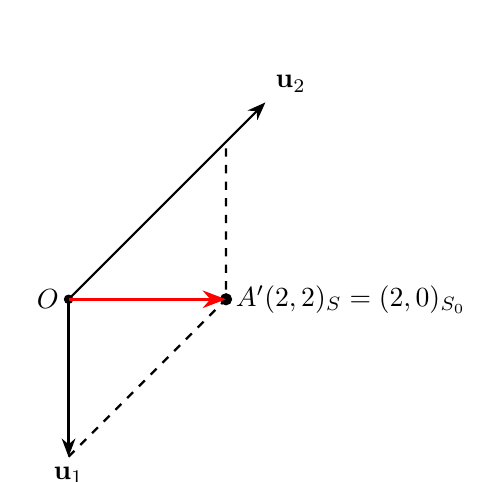
\begin{tikzpicture}[scale=1.0]
  \draw[thick, -Stealth] (0, 0) -- (0, -2) node[below] {$\mathbf{u}_1$};
  \draw[thick, -Stealth] (0, 0) -- (2.5, 2.5) node[above right] {$\mathbf{u}_2$};
  \filldraw (0, 0) circle (1.5pt) node[left] {$O$};

  \coordinate (Ap) at (2, 0);
  \filldraw (Ap) circle (2pt) node[right] {$A'(2, 2)_S = (2, 0)_{S_0}$};
  \draw[thick, dashed] (0, -2) -- (2, 0) -- (2, 2);
  \draw[very thick, -Stealth, red] (0, 0) -- (Ap);
\end{tikzpicture}
\caption{$A'$ 在新座標系下之向量分解}
\label{fig:b4-2-6}
\end{figure}

\subsubsection*{作業 6}
\begin{enumerate}[(i)]
  \item 在論例 1 中，求點 $B = (-1, 1), C = (-1, 0), D = (2, 5)$ 相關於座標系 $S$ 的座標．
  \item 在論例 1 中，求點 $B' = (1, -3)_S, C' = (-1, 3)_S, D' = (-3, -2)_S$ 相關於 $S_0$ 的座標．
\end{enumerate}

第三冊所比較的兩個不同座標系有一個特點，就是具有共同的原點，現在我們來看若原點改變，結果如何．

\begin{example}[例 3]
設 $S' \equiv (O'; \mathbf{u}_1, \mathbf{u}_2)$ 其基底與上論例相同，而 $\vec{OO'} = (3, -1)_{S_0}$．試求 $A(2, 1)$ 對 $S'$ 的座標及 $A'(2, 2)_{S'}$ 對 $S_0$ 的座標．
\end{example}

\begin{proof}[解]
設 $A = (x_1', x_2')_{S'}, A' = (x_1, x_2)_{S_0}$，則有
\begin{align*}
2\mathbf{i}_1 + 1\mathbf{i}_2 &= \vec{OA} = \vec{OO'} + \vec{O'A} \\
&= (3\mathbf{i}_1 - \mathbf{i}_2) + [x_1'(0\mathbf{i}_1 - 1\mathbf{i}_2) + x_2'(1\mathbf{i}_1 + 1\mathbf{i}_2)] \quad \text{〔由基底間的關係〕} \\
&= (3 + x_2')\mathbf{i}_1 + (-1 - x_1' + x_2')\mathbf{i}_2
\end{align*}
而有
\[ \begin{cases} 3 + x_2' = 2 \\ -1 - x_1' + x_2' = 1 \end{cases} \implies x_2' = -1, \; x_1' = -3 \]
故 $A = (2, 1) = (-3, -1)_{S'}$．

又
\begin{align*}
x_1\mathbf{i}_1 + x_2\mathbf{i}_2 &= \vec{OA'} = \vec{OO'} + \vec{O'A'} \\
&= (3\mathbf{i}_1 - \mathbf{i}_2) + [2(0\mathbf{i}_1 - 1\mathbf{i}_2) + 2(1\mathbf{i}_1 + 1\mathbf{i}_2)] \quad \text{〔由基底間的關係〕} \\
&= (3 + 2)\mathbf{i}_1 + (-1 - 2 + 2)\mathbf{i}_2 = 5\mathbf{i}_1 - 1\mathbf{i}_2
\end{align*}
$\therefore x_1 = 5, x_2 = -1$．故 $A' = (2, 2)_{S'} = (5, -1)_{S_0}$．
\end{proof}

\subsubsection*{作業 7}
取 $S'$ 如例 3，仿例 3 求作業 6 中各題．

\subsubsection*{作業 8}
試解釋在 \eqref{eq:b4-1-2-6} 式中 $\Delta \neq 0$（提示：參考第三冊 § 3-7 行列式與面積）．

總結本節結果，可得：

\begin{theorem}[定理 2]
給定平面上兩個座標系 $S \equiv (O; \mathbf{u}_1, \mathbf{u}_2)$ 及 $S' \equiv (O'; \mathbf{u}_1', \mathbf{u}_2')$ 如果
\begin{align*}
\mathbf{u}_1' &= a_{11}\mathbf{u}_1 + a_{12}\mathbf{u}_2 \\
\mathbf{u}_2' &= a_{21}\mathbf{u}_1 + a_{22}\mathbf{u}_2
\end{align*}
而且 $\vec{OO'} = b_1\mathbf{u}_1 + b_2\mathbf{u}_2$，則
\begin{equation}
\begin{cases}
x_1 = a_{11}x_1' + a_{21}x_2' + b_1 \\
x_2 = a_{12}x_1' + a_{22}x_2' + b_2
\end{cases} \label{eq:b4-1-2-thm2-5}
\end{equation}
或
\begin{equation}
\begin{cases}
x_1' = \dfrac{a_{22}(x_1 - b_1) - a_{21}(x_2 - b_2)}{\Delta} \\[1em]
x_2' = \dfrac{-a_{12}(x_1 - b_1) + a_{11}(x_2 - b_2)}{\Delta}
\end{cases} \label{eq:b4-1-2-thm2-6}
\end{equation}
其中 $\Delta = a_{11}a_{22} - a_{12}a_{21}$．
\end{theorem}

注意比較 \eqref{eq:b4-1-2-4} 與 \eqref{eq:b4-1-2-thm2-5} 式之一次部份：除 $a_{12}$ 與 $a_{21}$ 互調外，其餘相同．但注意 \eqref{eq:b4-1-2-4} 式將 $\mathbf{u}_1'$ 及 $\mathbf{u}_2'$ 以 $\mathbf{u}_1$ 及 $\mathbf{u}_2$ 表示，\eqref{eq:b4-1-2-thm2-5} 式則將 $x_1$ 及 $x_2$ 以 $x_1'$ 及 $x_2'$ 表示．

\vspace{1em}
\noindent\textbf{**【論例 2】（相對性原理）}\phantomsection\label{note:b4-ch1-p16-lorentz}\footnote{【原書註記/校訂】：原書標註「**【論例 2】（相對性原理）」，依目次「注意 1」規範，「**」表示本節段為選授/進階補充內容．}

平面上有兩同原點座標系 $S_0 \equiv (O; \mathbf{e}_1, \mathbf{e}_2), S \equiv (O; \mathbf{u}_1, \mathbf{u}_2)$，其中 $S_0$ 為正交座標系．設 $(x, t)$ 與 $(x', t')$ 分別為 $S_0$---座標與 $S$---座標，且其座標變換式為
\begin{equation}
\begin{cases}
x' = \dfrac{x - vt}{\sqrt{1 - \dfrac{v^2}{c^2}}} \\[1.5em]
t' = \dfrac{-\dfrac{v}{c^2}x + t}{\sqrt{1 - \dfrac{v^2}{c^2}}}
\end{cases} \label{eq:b4-lorentz-1}
\end{equation}
（稱羅倫茲（Lorentz）變換）其中 $c, v$ 皆為常數，求得兩組基底的關係應為（據 § I-2 \eqref{eq:b4-1-2-4} 及 \eqref{eq:b4-1-2-5} 式）
\begin{align*}
\mathbf{u}_1 &= \frac{\mathbf{e}_1 + \dfrac{v}{c^2}\mathbf{e}_2}{\sqrt{1 - \dfrac{v^2}{c^2}}} \\
\mathbf{u}_2 &= \frac{v\mathbf{e}_1 + \mathbf{e}_2}{\sqrt{1 - \dfrac{v^2}{c^2}}}
\end{align*}

今取平面上一點 $P$ 對一個靜坐在臺北站的觀測者甲看來 $P$ 可當作在 $t$ 時刻自臺北沿縱貫路南下 $x$ 公里處發生的一個事件，則相對論告訴我們，若有另一觀測者乙以等速度 $v$ 離甲（沿縱貫路）南去時，則剛才那一事件從乙看來應是 $t'$ 時刻在乙之南 $x'$ 公里處發生的事件．（$x'$ 為負時，代表事件發生在乙之北）．而這 $x', t'$ 與 $x, t$ 的關係由上述羅倫茲變換式給定，其中 $c$ 代表光速．

\begin{figure}[H]
\centering
\begin{tikzpicture}[scale=1.0]
  \draw[thick, -Stealth] (-0.5, 0) -- (4.5, 0) node[right] {$x$ ($\mathbf{e}_1$)};
  \draw[thick, -Stealth] (0, -0.5) -- (0, 4) node[above] {$t$ ($\mathbf{e}_2$)};
  \filldraw (0, 0) circle (1.5pt) node[below left] {$O$};

  % u1 (x') and u2 (t') axes (tilted)
  \draw[very thick, -Stealth, blue] (0, 0) -- (4.0, 1.4) node[right] {$x'$ ($\mathbf{u}_1$)};
  \draw[very thick, -Stealth, blue] (0, 0) -- (1.4, 4.0) node[above] {$t'$ ($\mathbf{u}_2$)};

  % Simultaneous line in S' (parallel to x' axis)
  \draw[thick, dashed, green!60!black] (0.2, 1.27) -- (4.2, 2.67) node[right] {\small $t' = \text{常數}$};

  % Events P1 and P2 on the simultaneous line
  \coordinate (P1) at (3.2, 2.32);
  \coordinate (P2) at (1.5, 1.725);
  \filldraw (P1) circle (2pt) node[above left] {$P_1(x_1', t')_S$};
  \filldraw (P2) circle (2pt) node[above left] {$P_2(x_2', t')_S$};

  % Projections to t-axis showing t1 != t2
  \draw[dotted, gray] (P1) -- (0, 2.32) node[left] {\footnotesize $t_1$};
  \draw[dotted, gray] (P2) -- (0, 1.725) node[left] {\footnotesize $t_2$};
\end{tikzpicture}
\caption{羅倫茲變換時空圖}
\label{fig:b4-2-7}
\end{figure}

相對論提出了幾點“新”的看法：
\begin{enumerate}[(i)]
  \item 它告訴我們傳統的所謂「同時」這一概念不是絕對的，而是依賴於觀測者的．解釋如下：取兩事件 $P_1(x_1', t')_S$ 與 $P_2(x_2', t')_S$．就是說，這兩事件從 $S$ 的乙觀測者看來，都發生在 $t'$ 時刻，是“同時的”，但根據變換式，這兩事件對 $S_0$ 的甲觀測者看來，則分別發生於不同時刻：
  \[ t_1 = \frac{\dfrac{v}{c^2}x_1' + t'}{\sqrt{1 - \dfrac{v^2}{c^2}}}, \qquad t_2 = \frac{\dfrac{v}{c^2}x_2' + t'}{\sqrt{1 - \dfrac{v^2}{c^2}}} \]
  兩事件發生的時差（對甲而言）為
  \[ t_1 - t_2 = \frac{\dfrac{v}{c^2}(x_1' - x_2')}{\sqrt{1 - \dfrac{v^2}{c^2}}} \]
  亦卽對甲而言，這兩事件並不“同時”．因此“同時”是一個相對性的概念．

  但注意當 $v$ 不是大到可與光速比較時，這時差非常細微，可以忽略不計．例如在日常或傳統的力學，如星體，砲彈，火箭等的相對運動下，「同時」仍有它逼近絕對性的意義．

  \item 設有一巨尺，其對靜止的甲看來長度為 $l$，將其自臺北站往南平放於縱貫路上，尺的兩端分別設一藍燈與紅燈，使其持續發光，則發藍光與發紅光為兩整串的事件，在 $(x, t)$ 平面上分別描出
  \[ x = 0, \qquad x = l \]
  兩條直線（半射線）．

  今乙觀測者要測此巨尺的長度，設他觀測的時刻為 $t'$，則 $t'$ 時刻他“看到的”藍光與紅光的位置 $x_1', x_2'$ 其差距 $x_2' - x_1'$ 卽為他所測得的尺長 $l'$．

  由 \eqref{eq:b4-lorentz-1} 式，解得其 $x, t$ 表為 $x', t'$ 的座標變換式為（作業 9）：
  \begin{equation}
  \begin{cases}
  x = \dfrac{x' + vt'}{\sqrt{1 - \dfrac{v^2}{c^2}}} \\[1.5em]
  t = \dfrac{\dfrac{v}{c^2}x' + t'}{\sqrt{1 - \dfrac{v^2}{c^2}}}
  \end{cases} \label{eq:b4-lorentz-2}
  \end{equation}
  其相應的 $S_0$ 的第一座標為：$x_1 = 0, x_2 = l$．

  \begin{figure}[H]
  \centering
  \begin{tikzpicture}[scale=1.05]
    \draw[thick, -Stealth] (-0.5, 0) -- (4.2, 0) node[right] {$x$};
    \draw[thick, -Stealth] (0, -0.5) -- (0, 4.2) node[above] {$t$};
    \filldraw (0, 0) circle (1.5pt) node[below left] {$O$};

    % World lines x=0 and x=l
    \draw[very thick, blue] (0, 0) -- (0, 3.8) node[above] {\small $x=0$ (藍光)};
    \draw[very thick, red] (2.6, 0) -- (2.6, 3.8) node[above] {\small $x=l$ (紅光)};
    \draw[|<->|] (0, -0.4) -- (2.6, -0.4) node[midway, fill=white, inner sep=1pt] {\small $l$};

    % Line of constant t'
    \draw[thick, dashed, green!60!black] (-0.5, 0.8) -- (3.8, 2.2) node[right] {\small $t' = \text{常數}$};
    \filldraw (0, 0.96) circle (2pt) node[above left] {$x_1'$};
    \filldraw (2.6, 1.8) circle (2pt) node[below right] {$x_2'$};
    \draw[|<->|, purple] ($(0, 0.96) + (-0.1, 0.25)$) -- ($(2.6, 1.8) + (-0.1, 0.25)$) node[midway, above left] {\small $l'$};
  \end{tikzpicture}
  \caption{長度測量與尺縮效應}
  \label{fig:b4-2-8}
  \end{figure}

  由 \eqref{eq:b4-lorentz-2} 中第一式：
  \[ x_1 = \frac{x_1' + vt'}{\sqrt{1 - \dfrac{v^2}{c^2}}} = 0 \implies x_1' = -vt' \]
  \[ x_2 = \frac{x_2' + vt'}{\sqrt{1 - \dfrac{v^2}{c^2}}} = l \implies x_2' + vt' = l\sqrt{1 - \frac{v^2}{c^2}} \implies x_2' = l\sqrt{1 - \frac{v^2}{c^2}} - vt' \]
  故
  \[ l' = x_2' - x_1' = l\sqrt{1 - \frac{v^2}{c^2}} \]
  故從乙看來，該尺竟然自 $l$ 壓縮了 $\sqrt{1 - \dfrac{v^2}{c^2}}$ 倍，卽得尺長 $l\sqrt{1 - \dfrac{v^2}{c^2}}$．這就稱為「長度的壓縮性」（或空間的壓縮性）．
\end{enumerate}

\subsubsection*{作業 9}
試由 \eqref{eq:b4-lorentz-1} 式解得 \eqref{eq:b4-lorentz-2} 式．

\subsubsection*{作業 10}
如果兩觀測者的相對速度與光速 $c$ 相較甚小，則傳統力學適用（此時 $\dfrac{v}{c}$ 與 $\dfrac{v^2}{c^2}$ 皆甚小）．解釋此時 \eqref{eq:b4-lorentz-1} 式的意義．

\subsubsection*{作業 11}
甲觀測系統的尺度，由乙看來壓縮了 $\sqrt{1 - \dfrac{v^2}{c^2}}$ 倍，反過來乙的尺度甲看起來應為伸漲或壓縮？其漲縮率為何？

\subsubsection*{習題 1-2}
\begin{enumerate}
  \item 在平面上取一自然座標系 $S_0 \equiv (O; \mathbf{i}_1, \mathbf{i}_2)$，假設有一點 $P$ 用此座標系表示時 $P = (1, 0)$．令
  \begin{enumerate}[a.]
    \item $A = (1, 1), B = (-1, 1)$
    \item $A = (0, 1), B = (\frac{1}{2}, \frac{1}{2})$
    \item $A = (\frac{1}{2}, 5), B = (-\frac{3}{5}, -6)$
  \end{enumerate}
  問：
  \begin{enumerate}[(i)]
    \item 上述各種情形中 $(O; \vec{OA}, \vec{OB})$ 是不是可以形成一座標系？
    \item 上述各種情形中 $(P; \vec{PA}, \vec{PB})$ 可不可以成為一個座標系？
  \end{enumerate}

  \item 設 $S \equiv (O; \mathbf{u}_1, \mathbf{u}_2)$ 為平面 $\mathbf{R}^2$ 上的一個座標系，現在有 $\mathbf{R}^2$ 上的三點 $O', A, B$ 用此座標系表示為：$O' = (1, 1)_S, A = (\sqrt{2}, 5)_S, B = (4, -1)_S$．令 $\mathbf{u}_1' = \vec{O'A}, \mathbf{u}_2' = \vec{O'B}$，問：
  \begin{enumerate}[(i)]
    \item $S' \equiv (O'; \mathbf{u}_1', \mathbf{u}_2')$ 是不是可成為一個座標系？
    \item 如果 $S' \equiv (O'; \mathbf{u}_1', \mathbf{u}_2')$ 是個座標系，則由 $S$ 變換成 $S'$ 的座標變換如何表示？
  \end{enumerate}

  \item 把地球表面看成一個平面，以臺北做原點 $O$，以向東 $1$ 公里的向量 $\mathbf{e}_1$ 及向北 $1$ 公里的向量 $\mathbf{e}_2$ 為基底得一座標系．香港因為目前是英國屬地，以英制的哩為單位，故在香港 $O'$ 可以拿向東 $1$ 哩的向量 $\mathbf{e}_1'$ 及向北 $1$ 哩的向量 $\mathbf{e}_2'$ 做基底得另一座標系，現已知香港是在臺北的西方 $800$ 公里，如果有一艘船在海上，由臺北的座標來看，它的位置是在 $(-300, 200)$ 處．由香港做原點的座標系來看，它的位置應該如何表示？（$1$ 哩 $= 1.6093$ 公里）．

  \item 如果有一天，我國收回了香港，當然香港的度量衡也改為公制了．香港的里程也就以公里來計算，則上題的答案如何？

  \item 有一同學在操場上沿一直線跑步，現假設操場為一平面，以公尺為長度單位，在他起跑點 $O$ 做一座標系 $(O; \mathbf{e}_1, \mathbf{e}_2)$．他跑步的速度如用向量表示為每秒鐘 $\mathbf{v} = 3\mathbf{e}_1 + 4\mathbf{e}_2$．在他跑步的每一瞬間用他當時的位置做原點，用同樣的 $\mathbf{e}_1, \mathbf{e}_2$ 做基底可得一座標系，如此我們就得到了一個在操場上移動的座標系，現操場上有一個國旗桿，它的位置若用跑到 $10$ 秒時的座標系來表示是 $(20, 30)$ 問用跑到 $25$ 秒時的座標系應該如何表示？兩個座標系之間如何變換？

  \item 設有一火車在軌道上沿一直線作等速運動，設在時刻 $t$ 火車的位置為 $O_t$，我們固定兩個方向 $\mathbf{e}_1, \mathbf{e}_2$ 作基底，則在任意時刻 $t$，均有一座標系 $(O_t; \mathbf{e}_1, \mathbf{e}_2) \equiv S_t$．因火車在每一秒鐘均走一固定的向量 $\mathbf{v}$，設 $\mathbf{v} = 5\mathbf{e}_1$，當時刻 $t = 0$ 時，我們看見有一房屋，對 $S_0$ 是在 $(0, 2)$ 的位置，試問在時刻 $t$ 時，相對於 $S_t$ 座標系，該房屋的座標應為多少？（讀者會發現在每個時刻 $t$，房屋所對應於 $S_t$ 的座標均不同，此卽何以我們在車輛中感覺到車外的房屋一直在動的原因）．
\end{enumerate}
% =========================================================================
% § I-3 平面上的線性映射
% =========================================================================
\subsection{平面上的線性映射}
\label{sec:b4-1-3}

本段將固定採用自然座標系 $S_0$．

\subsubsection*{甲、線性映射的意義}

上節（§ I-2）座標變換的式子 \eqref{eq:b4-1-2-5}
\begin{align*}
x_1 &= a_{11}x_1' + a_{21}x_2' + b_1 \\
x_2 &= a_{12}x_1' + a_{22}x_2' + b_2
\end{align*}
及 § I-1 的 (3)（或 (3')）
\[ x = ax' + b \]
使我們想起實數系 $\mathbf{R} = \mathbf{R}^1$〔註〕的一次變換
\begin{equation}
y = ax + b \label{eq:b4-1-3-1}
\end{equation}
亦卽考慮一次函數 $f: \mathbf{R}^1 \to \mathbf{R}^1$ 其中
\begin{equation}
f(x) = ax + b \label{eq:b4-1-3-2}
\end{equation}
這種函數在自然或人文現象的各種函數關係中最是單純，我們已從第三冊學得它可以圖解如下：

\begin{figure}[H]
\centering
\begin{tikzpicture}[scale=1.0]
  \draw[thick, -Stealth] (-1, 0) -- (4, 0) node[right] {$x$};
  \draw[thick, -Stealth] (0, -1) -- (0, 3.5) node[above] {$y$};
  \filldraw (0, 0) circle (1.5pt) node[below left] {$O$};

  \draw[very thick, blue] (-0.5, 0.5) -- (3.5, 3.1) node[right] {$y = ax + b$};
  \filldraw (0, 0.83) circle (1.5pt) node[left] {$b$};
  \node at (2.5, 1.5) {\small $a$ 代表這直線的斜率};
  \node at (2.5, 1.0) {\small $b$ 代表 $y$ 截距};
\end{tikzpicture}
\caption{一次函數之圖形}
\label{fig:b4-1-3-1}
\end{figure}

〔註〕實數軸上點變動的自由度為 $1$，我們把實數系看成是 $1$ 維的，所以寫成 $\mathbf{R}^1$．平面上點變動的自由度為 $2$，我們把平面看成 $\mathbf{R} \times \mathbf{R}$，將寫成 $\mathbf{R}^2$．

現在將 \eqref{eq:b4-1-3-1} 式寫成
\begin{equation}
\begin{cases}
y_1 = a_{11}x_1 + a_{21}x_2 + b_1 \\
y_2 = a_{12}x_1 + a_{22}x_2 + b_2
\end{cases} \label{eq:b4-1-3-3}
\end{equation}
\eqref{eq:b4-1-3-3} 式可以看成：兩變量 $y_1$ 與 $y_2$ 相應於兩變量 $x_1$ 及 $x_2$ 的變化關係，就這立場，我們慣以函數稱之．但當我們把 $(x_1, x_2), (y_1, y_2)$ 都看成平面上的點時，我們注重的是平面上點的位置變動的情形，此時慣以映射稱之．〔見章末附註〕

這一節我們特別注重函數的幾何意義，而因 \eqref{eq:b4-1-3-3} 式所給的函數是一次的，我們先考慮所謂的“線性映射”：

\begin{definition}[定義]
設 $f: \mathbf{R}^2 \to \mathbf{R}^2$ 為一函數，以 $(y_1, y_2)$ 表 $(x_1, x_2)$ 在 $f$ 下之像點，而知存在四實數 $a_{11}, a_{12}, a_{21}, a_{22}$，使得
\begin{equation}
\begin{cases}
y_1 = a_{11}x_1 + a_{21}x_2 \\
y_2 = a_{12}x_1 + a_{22}x_2
\end{cases} \label{eq:b4-1-3-4}
\end{equation}
對每一點 $(x_1, x_2)$ 都成立，則稱 $f$ 為 $\mathbf{R}^2$ 到 $\mathbf{R}^2$ 的一個線性映射．（注意：$y_1$ 與 $y_2$ 均為 $x_1$ 與 $x_2$ 的一次齊次函數）
\end{definition}

\begin{figure}[H]
\centering
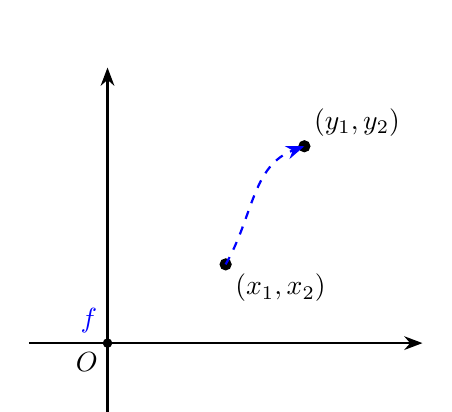
\begin{tikzpicture}[scale=1.0]
  \draw[thick, -Stealth] (-1, 0) -- (4, 0);
  \draw[thick, -Stealth] (0, -1) -- (0, 3.5);
  \filldraw (0, 0) circle (1.5pt) node[below left] {$O$};

  \filldraw (1.5, 1.0) circle (2pt) node[below right] {$(x_1, x_2)$};
  \filldraw (2.5, 2.5) circle (2pt) node[above right] {$(y_1, y_2)$};
  \draw[thick, -Stealth, dashed, blue] (1.5, 1.0) to[out=60, in=200] (2.5, 2.5) node[midway, above left] {$f$};
\end{tikzpicture}
\caption{線性映射示意圖}
\label{fig:b4-1-3-2}
\end{figure}

這樣定義得來的線性映射可寫成：
\begin{equation}
f(x_1, x_2) = (a_{11}x_1 + a_{21}x_2, \; a_{12}x_1 + a_{22}x_2) \label{eq:b4-1-3-5}
\end{equation}

\noindent\textbf{注意}：線性映射是把平面的點移到新的位置，而座標變換的意義則是固定平面上的點，只按照新舊座標間的關係來改寫平面上點的座標表示．當兩座標系之原點合一時，線性映射與座標變換的代數式一樣，兩方面的推論結果可相互轉化來利用，但注意就其自然的意義來看兩者是有著區別的．

\begin{example}[例 4]
已知線性映射 $f$ 由下式給出：
\[ \begin{cases} y_1 = 3x_1 - x_2 \\ y_2 = 2x_1 + x_2 \end{cases} \]
求 $O(0, 0), A(2, 0), B(1, 1), C(0, 2)$ 相應之像點 $O', A', B', C'$ 的座標，又 $A, B, C$ 三點同在一直線上，問 $A', B', C'$ 是否也同在一直線上？
\end{example}

\begin{proof}[解]
計算易知 $f(0, 0) = (0, 0), f(1, 1) = (2, 3), f(2, 0) = (6, 4), f(0, 2) = (-2, 2)$．故 $A' = (6, 4), B' = (2, 3), C' = (-2, 2)$．

檢驗三點 $A', B', C'$ 是否共線的方法很多，由 $\vec{A'B'} = (-4, -1), \vec{B'C'} = (-4, -1)$ 可知共線，或由行列式
\[ \begin{vmatrix} 6 & 4 & 1 \\ 2 & 3 & 1 \\ -2 & 2 & 1 \end{vmatrix} = 0 \]
亦可知（第三冊 § 4-2 論例 3）．
\end{proof}

\subsubsection*{作業 12}
對於自然座標系 $S_0$，四點 $A(-1, -1), B(3, 1), C(1, 5), D(-3, 3)$ 做成一正方形的頂點（為什麼？試先檢驗）．
\begin{enumerate}[(i)]
  \item 求在例 4 的線性映射下，此四點的像點．
  \item 此四像點仍做成一正方形的頂點嗎？或為一矩形？或只得一平行四邊形？甚或僅為一任意四邊形而已？
  \item 試求基底向量的終點的像點，並由像點的座標寫出基底經線性映射後變成的新向量 $\mathbf{u}_1, \mathbf{u}_2$，試問四像點，對應於 $S \equiv (O; \mathbf{u}_1, \mathbf{u}_2)$ 的座標如何？（此題表示一般的線性映射不保持角度也不保持長度）．
\end{enumerate}

\subsubsection*{乙、線性映射的基本性質}

我們已在例 4 中看出在線性映射下原點的像點仍為原點．

線性映射既然是一個把平面上的點指向其像點的函數，自然能把平面上的向量（先看成自原點出發的）指向以原點為起點，以其終點之像點為終點的向量．若 $P$ 為點 $(x_1, x_2)$，$Q$ 表 $P$ 經 $f$ 的像點，則有兩種寫法：$f(P) = Q$ 或 $f(\vec{OP}) = \vec{OQ}$．

也就是說：若 $f: \mathbf{R}^2 \to \mathbf{R}^2$ 為線性映射，則 $f(\vec{OP}) = \vec{OQ}$，其中 $Q$ 為 $P$ 經 $f$ 的像點．我們利用平面的點與自某定點出發以之為終點的向量的一一對應，有時把 $f$ 的定義域 $\mathbf{R}^2$ 中的元素看成點，有時又把 $\mathbf{R}^2$ 的元素看成向量，事實上點的座標與其相應向量的座標成分是一樣的，故為了不同需要可以寫 $f(P) = Q$，亦可寫 $f(\vec{OP}) = \vec{OQ}$．

$\mathbf{R}^2$ 中的元素既然可以看成向量，而向量在本質上是可以不計其起始點的，因此對任給向量 $\mathbf{a}$，$f(\mathbf{a})$ 也就有了一定的意思，卽：$f(\mathbf{a})$ 是以 $\mathbf{a}$ 的始點之像點為始點，$\mathbf{a}$ 終點之像點為終點的向量，稱為向量 $\mathbf{a}$ 的映像．

第三冊 § 5-1 提到空間中自同一點出發的兩個線性無關向量 $\mathbf{a}$ 與 $\mathbf{b}$ 可張出一平面 $P$，而此平面又可依據此二向量為基底，共同始點為原點做成其上的一座標系．設共同出發點為 $O$，則 $P = \{P \mid \vec{OP} = \alpha\mathbf{a} + \beta\mathbf{b}\}$，我們稱向量 $\vec{OP}$ 為 $\mathbf{a}$ 與 $\mathbf{b}$ 的線性組合，此組合的係數卽為此點相關於座標系 $S \equiv (O; \mathbf{a}, \mathbf{b})$ 的座標．

由以上的觀點，甲段所述的線性映射（\eqref{eq:b4-1-3-4} 式）有一可以不藉座標便能表達的特徵性質，卽：平面上兩向量的線性組合，經線性映射後的映像，為此兩向量的映像的線性組合．

\begin{theorem}[定理 3]
若 $f: \mathbf{R}^2 \to \mathbf{R}^2$ 為一線性映射，則對於任意兩實數 $\alpha, \beta \in \mathbf{R}^1$ 及任意平面上的兩向量 $\mathbf{a}$ 與 $\mathbf{b}$ 總有
\begin{equation}
f(\alpha\mathbf{a} + \beta\mathbf{b}) = \alpha f(\mathbf{a}) + \beta f(\mathbf{b}) \label{eq:b4-1-3-6}
\end{equation}
（\eqref{eq:b4-1-3-6} 式的性質，稱為函數 $f$ 的線性條件）．
\end{theorem}

\begin{proof}[證明]
設 $\mathbf{a} = (x_1, x_2), \mathbf{b} = (x_1', x_2')$，則 $\alpha\mathbf{a} + \beta\mathbf{b} = (\alpha x_1 + \beta x_1', \alpha x_2 + \beta x_2')$．故由 \eqref{eq:b4-1-3-4} 式：
\begin{align*}
f(\alpha\mathbf{a} + \beta\mathbf{b}) &= (a_{11}(\alpha x_1 + \beta x_1') + a_{21}(\alpha x_2 + \beta x_2'), \; a_{12}(\alpha x_1 + \beta x_1') + a_{22}(\alpha x_2 + \beta x_2')) \\
&= \alpha(a_{11}x_1 + a_{21}x_2, a_{12}x_1 + a_{22}x_2) + \beta(a_{11}x_1' + a_{21}x_2', a_{12}x_1' + a_{22}x_2') \\
&= \alpha f(\mathbf{a}) + \beta f(\mathbf{b})
\end{align*}
\end{proof}

\eqref{eq:b4-1-3-6} 式這一個性質非常基本，特別地：
\begin{enumerate}[(i)]
  \item 取 $\alpha = 1, \beta = 1$，得 $f(\mathbf{a} + \mathbf{b}) = f(\mathbf{a}) + f(\mathbf{b})$（保加法性，圖 \ref{fig:b4-1-3-3}）．
  \item 取 $\beta = 0$，得 $f(\alpha\mathbf{a}) = \alpha f(\mathbf{a})$（保係數積，圖 \ref{fig:b4-1-3-4}）．
  \item 取 $\alpha = 0, \beta = 0$，得 $f(\mathbf{0}) = \mathbf{0}$（原點不變）．
  \item 取 $\alpha = 1, \beta = -1$，得 $f(\mathbf{a} - \mathbf{b}) = f(\mathbf{a}) - f(\mathbf{b})$．
\end{enumerate}

\begin{figure}[H]
\centering
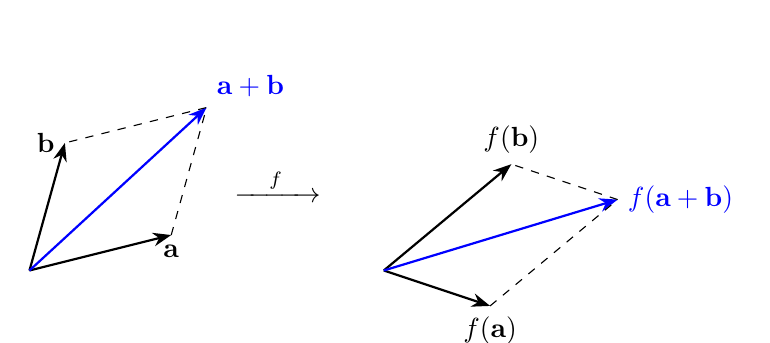
\begin{tikzpicture}[scale=0.9]
  % Addition
  \draw[thick, -Stealth] (0, 0) -- (2, 0.5) node[below] {$\mathbf{a}$};
  \draw[thick, -Stealth] (0, 0) -- (0.5, 1.8) node[left] {$\mathbf{b}$};
  \draw[thick, -Stealth, blue] (0, 0) -- (2.5, 2.3) node[above right] {$\mathbf{a}+\mathbf{b}$};
  \draw[dashed] (2, 0.5) -- (2.5, 2.3) -- (0.5, 1.8);

  \node at (3.5, 1.2) {$\xrightarrow{\quad f \quad}$};

  \begin{scope}[shift={(5, 0)}]
    \draw[thick, -Stealth] (0, 0) -- (1.5, -0.5) node[below] {$f(\mathbf{a})$};
    \draw[thick, -Stealth] (0, 0) -- (1.8, 1.5) node[above] {$f(\mathbf{b})$};
    \draw[thick, -Stealth, blue] (0, 0) -- (3.3, 1.0) node[right] {$f(\mathbf{a}+\mathbf{b})$};
    \draw[dashed] (1.5, -0.5) -- (3.3, 1.0) -- (1.8, 1.5);
  \end{scope}
\end{tikzpicture}
\caption{線性映射保持向量加法}
\label{fig:b4-1-3-3}
\end{figure}

\begin{figure}[H]
\centering
\begin{tikzpicture}[scale=0.9]
  \draw[thick, -Stealth] (0, 0) -- (1.5, 0.8) node[above] {$\mathbf{a}$};
  \draw[very thick, -Stealth, blue] (0, 0) -- (3.0, 1.6) node[right] {$\alpha\mathbf{a}$};

  \node at (4.0, 0.8) {$\xrightarrow{\quad f \quad}$};

  \begin{scope}[shift={(5.5, 0)}]
    \draw[thick, -Stealth] (0, 0) -- (1.2, -0.6) node[below] {$f(\mathbf{a})$};
    \draw[very thick, -Stealth, blue] (0, 0) -- (2.4, -1.2) node[right] {$f(\alpha\mathbf{a}) = \alpha f(\mathbf{a})$};
  \end{scope}
\end{tikzpicture}
\caption{線性映射保持純量積}
\label{fig:b4-1-3-4}
\end{figure}

\subsubsection*{作業 13}
若 $f$ 滿足 $f(\mathbf{a} + \mathbf{b}) = f(\mathbf{a}) + f(\mathbf{b})$ 及 $f(\alpha\mathbf{a}) = \alpha f(\mathbf{a})$，試證 $f(\alpha\mathbf{a} + \beta\mathbf{b}) = \alpha f(\mathbf{a}) + \beta f(\mathbf{b})$．

\subsubsection*{作業 14}
利用數學歸納法證明：若 $f: \mathbf{R}^2 \to \mathbf{R}^2$ 為線性映射，則對任意 $k$ 個向量 $\mathbf{a}_1, \dots, \mathbf{a}_k$ 及 $k$ 個實數 $\alpha_1, \dots, \alpha_k$ 恆有
\[ f\left(\sum_{i=1}^k \alpha_i \mathbf{a}_i\right) = \sum_{i=1}^k \alpha_i f(\mathbf{a}_i) \]

\subsubsection*{丙、線性映射的矩陣表示}

設 $S \equiv (O; \mathbf{u}_1, \mathbf{u}_2)$ 為平面上任一座標系，則平面上任一向量 $\mathbf{v}$ 可唯一表成 $\mathbf{v} = \alpha\mathbf{u}_1 + \beta\mathbf{u}_2$．若知 $\mathbf{u}_1, \mathbf{u}_2$ 在線性映射 $f$ 下之像向量為
\begin{align}
\mathbf{u}_1' &= f(\mathbf{u}_1) = a_{11}\mathbf{u}_1 + a_{12}\mathbf{u}_2 \label{eq:b4-1-3-7} \\
\mathbf{u}_2' &= f(\mathbf{u}_2) = a_{21}\mathbf{u}_1 + a_{22}\mathbf{u}_2 \nonumber
\end{align}
則由線性條件，
\[ f(\mathbf{v}) = f(\alpha\mathbf{u}_1 + \beta\mathbf{u}_2) = \alpha f(\mathbf{u}_1) + \beta f(\mathbf{u}_2) = \alpha\mathbf{u}_1' + \beta\mathbf{u}_2' \]
也就是說：只要知道基底向量 $\mathbf{u}_1, \mathbf{u}_2$ 的映像 $\mathbf{u}_1', \mathbf{u}_2'$，則全平面任何向量的映像便完全被確定了！

\begin{figure}[H]
\centering
\begin{tikzpicture}[scale=0.95]
  % Domain
  \coordinate (O) at (0, 0);
  \coordinate (U1) at (1.5, 0);
  \coordinate (U2) at (0.4, 1.5);
  \draw[thick, -Stealth] (O) -- (2.6, 0) node[below right] {$\mathbf{u}_1$};
  \draw[thick, -Stealth] (O) -- (0.7, 2.4) node[above left] {$\mathbf{u}_2$};
  \filldraw (O) circle (1.5pt) node[below left] {$O$};

  \coordinate (P) at ($1.3*(U1) + 1.1*(U2)$);
  \filldraw (P) circle (1.5pt) node[above right] {$P(\alpha, \beta)_S$};
  \draw[thick, dashed, blue] (O) -- (P);
  \draw[densely dotted, gray] (P) -- ($1.3*(U1)$);
  \draw[densely dotted, gray] (P) -- ($1.1*(U2)$);

  \node at (3.5, 1.2) {$\xrightarrow{\quad f \quad}$};

  % Codomain
  \begin{scope}[shift={(5.2, 0)}]
    \coordinate (Op) at (0, 0);
    \coordinate (U1p) at (1.4, -0.4);
    \coordinate (U2p) at (0.6, 1.6);
    \draw[thick, -Stealth, red] (Op) -- (2.3, -0.66) node[below right] {$\mathbf{u}_1' = f(\mathbf{u}_1)$};
    \draw[thick, -Stealth, red] (Op) -- (1.0, 2.6) node[above left] {$\mathbf{u}_2' = f(\mathbf{u}_2)$};
    \filldraw (Op) circle (1.5pt) node[below left] {$O$};

    \coordinate (Pp) at ($1.3*(U1p) + 1.1*(U2p)$);
    \filldraw (Pp) circle (1.5pt) node[above right] {$P' = f(P)$};
    \draw[thick, dashed, red] (Op) -- (Pp);
    \draw[densely dotted, gray] (Pp) -- ($1.3*(U1p)$);
    \draw[densely dotted, gray] (Pp) -- ($1.1*(U2p)$);
  \end{scope}
\end{tikzpicture}
\caption{基底向量之映射決定全體映射}
\label{fig:b4-1-3-5}
\end{figure}

這四個實數 $a_{11}, a_{12}, a_{21}, a_{22}$ 排成一個二列二行的數表：
\begin{equation}
[f]_S = \begin{pmatrix} a_{11} & a_{21} \\ a_{12} & a_{22} \end{pmatrix}_S \label{eq:b4-1-3-8}
\end{equation}
稱為線性映射 $f$ 相關於座標系 $S$ 的矩陣表示，記為 $[f]_S$．特殊地，當 $S$ 取為自然座標系 $S_0$ 時，矩陣表示簡記為 $[f]$，稱為 $f$ 的自然矩陣表示：
\[ [f] = \begin{pmatrix} a_{11} & a_{21} \\ a_{12} & a_{22} \end{pmatrix} \]

\begin{example}[例 5]
試求作業 12 中 $f$ 的自然矩陣表示．
\end{example}

\begin{proof}[解]
先看自然基底經 $f$ 的寫像：
由 $f(1, 0) = (3, 2)$ 可知 $f(\mathbf{i}_1) = 3\mathbf{i}_1 + 2\mathbf{i}_2$．
由 $f(0, 1) = (-1, 1)$ 可知 $f(\mathbf{i}_2) = -1\mathbf{i}_1 + 1\mathbf{i}_2$．
故自然矩陣表示為
\[ [f] = \begin{pmatrix} 3 & -1 \\ 2 & 1 \end{pmatrix} \]
\end{proof}

\subsubsection*{作業 15}
上文中若 $A_1, A_2$ 之自然座標按序為 $(1, 0), (0, 2)$．今知 $A_1, A_2$ 經過 $f$ 的像點 $A_1', A_2'$ 之自然座標按序為 $(1, 2), (-1, 1)$．問 $P = (1.5, 0.5)$ 之像點 $P'$ 自然座標為何？又若表為 \eqref{eq:b4-1-3-7} 式，則四實數 $a_{11}, a_{12}, a_{21}, a_{22}$ 應各為若干？

\subsubsection*{作業 16}
作業 12 中取 $\vec{OA}_1 = \mathbf{u}_1, \vec{OA}_2 = \mathbf{u}_2$，設 $S \equiv (O; \mathbf{u}_1, \mathbf{u}_2)$，問 $f$ 相關於 $S$ 之矩陣表示如何？

\subsubsection*{丁、線性映射的聯立式}

一個線性映射 $f$ 依甲段定義能表成下式：
\begin{equation}
\begin{cases}
y_1 = a_{11}x_1 + a_{21}x_2 \\
y_2 = a_{12}x_1 + a_{22}x_2
\end{cases} \label{eq:b4-1-3-9}
\end{equation}
其中 $(y_1, y_2), (x_1, x_2)$ 皆以自然座標表之．

但這樣的型式不只採取自然座標系 $S_0$ 時才成立．實際上對任一線性映射 $f: \mathbf{R}^2 \to \mathbf{R}^2$ 及任一座標系 $S \equiv (O; \mathbf{u}_1, \mathbf{u}_2)$，$f$ 都可以這樣來表示，這是本段要說明的．

\begin{figure}[H]
\centering
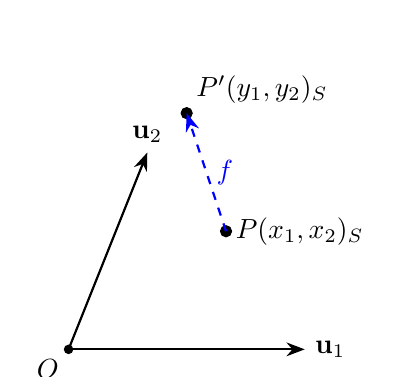
\begin{tikzpicture}[scale=1.0]
  \draw[thick, -Stealth] (0, 0) -- (3, 0) node[right] {$\mathbf{u}_1$};
  \draw[thick, -Stealth] (0, 0) -- (1, 2.5) node[above] {$\mathbf{u}_2$};
  \filldraw (0, 0) circle (1.5pt) node[below left] {$O$};
  \filldraw (2, 1.5) circle (2pt) node[right] {$P(x_1, x_2)_S$};
  \filldraw (1.5, 3.0) circle (2pt) node[above right] {$P'(y_1, y_2)_S$};
  \draw[thick, dashed, blue, -Stealth] (2, 1.5) -- (1.5, 3.0) node[midway, right] {$f$};
\end{tikzpicture}
\caption{一般座標系下的線性映射}
\label{fig:b4-1-3-6}
\end{figure}

\begin{proposition}[命題 2]
給定一線性映射 $f$，設 $S \equiv (O; \mathbf{u}_1, \mathbf{u}_2)$，$P = (x_1, x_2)_S$ 經 $f$ 的像點 $P'$ 的座標為 $(y_1, y_2)_S$，則兩座標的關係式為：
\begin{equation}
\begin{cases}
y_1 = a_{11}x_1 + a_{21}x_2 \\
y_2 = a_{12}x_1 + a_{22}x_2
\end{cases} \label{eq:b4-1-3-11}
\end{equation}
〔此稱為 $f$ 的座標表示式〕，其中 $(a_{ij})$ 為 $f$ 根據 $S$ 的矩陣表示，亦卽
\begin{align*}
f(\mathbf{u}_1) &= a_{11}\mathbf{u}_1 + a_{12}\mathbf{u}_2 \\
f(\mathbf{u}_2) &= a_{21}\mathbf{u}_1 + a_{22}\mathbf{u}_2
\end{align*}
\end{proposition}

\begin{theorem}[定理 4]
任一滿足“線性條件”（\eqref{eq:b4-1-3-6} 式）之 $f: \mathbf{R}^2 \to \mathbf{R}^2$ 必為一線性映射，亦卽其自然座標間的關係可表成 \eqref{eq:b4-1-3-4} 式．
\end{theorem}

\begin{example}[例 6]
設線性映射把 $\mathbf{u}_1 = (1, 1)$ 與 $\mathbf{u}_2 = (2, -1)$ 分別映像至 $f(\mathbf{u}_1) = (1, 0), f(\mathbf{u}_2) = (0, 1)$．試求 $f$ 相關於 $S$ 的座標表示式，並求 $P = (5, -2)_S$ 及 $Q = (-2, 5)_S$ 的像點，其中 $S \equiv (O; \mathbf{u}_1, \mathbf{u}_2)$．
\end{example}

\begin{proof}[解]
先求聯立式中之 $a_{ij}$：
\begin{align*}
(1, 0) &= a_{11}(1, 1) + a_{12}(2, -1) \implies \begin{cases} a_{11} + 2a_{12} = 1 \\ a_{11} - a_{12} = 0 \end{cases} \implies a_{11} = \frac{1}{3}, \; a_{12} = \frac{1}{3} \\
(0, 1) &= a_{21}(1, 1) + a_{22}(2, -1) \implies \begin{cases} a_{21} + 2a_{22} = 0 \\ a_{21} - a_{22} = 1 \end{cases} \implies a_{21} = \frac{2}{3}, \; a_{22} = -\frac{1}{3}
\end{align*}
故 $[f]_S = \begin{pmatrix} \frac{1}{3} & \frac{2}{3} \\ \frac{1}{3} & -\frac{1}{3} \end{pmatrix}_S$．座標表示式為：
\[ \begin{cases} y_1 = \frac{1}{3}x_1 + \frac{2}{3}x_2 \\ y_2 = \frac{1}{3}x_1 - \frac{1}{3}x_2 \end{cases} \]
代入得 $P' = (\frac{1}{3}, \frac{7}{3})_S, Q' = (\frac{8}{3}, -\frac{7}{3})_S$．
\end{proof}

\begin{figure}[H]
\centering
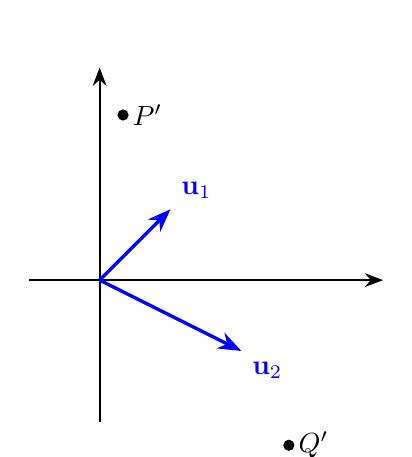
\begin{tikzpicture}[scale=0.9]
  \draw[thick, -Stealth] (-1, 0) -- (4, 0);
  \draw[thick, -Stealth] (0, -2) -- (0, 3);
  \draw[very thick, -Stealth, blue] (0, 0) -- (1, 1) node[above right] {$\mathbf{u}_1$};
  \draw[very thick, -Stealth, blue] (0, 0) -- (2, -1) node[below right] {$\mathbf{u}_2$};
  \filldraw (0.33, 2.33) circle (2pt) node[right] {$P'$};
  \filldraw (2.67, -2.33) circle (2pt) node[right] {$Q'$};
\end{tikzpicture}
\caption{例 6 之像點位置}
\label{fig:b4-1-3-7}
\end{figure}

\begin{example}[例 7]
設 $S \equiv (O; \mathbf{u}_1, \mathbf{u}_2), \mathbf{u}_1 = (1, 1), \mathbf{u}_2 = (2, -1)$，線性映射 $f$ 相關於 $S$ 的座標表示式為 $f(x_1, x_2)_S = (3x_1 - x_2, 2x_1 + x_2)_S$．試求 $\mathbf{u}_1 = (1, 1), \mathbf{u}_2 = (2, -1)$ 經 $f$ 的映像．
\end{example}

\begin{proof}[解]
求 $\mathbf{u}_1, \mathbf{u}_2$ 經 $f$ 的映像卽在求點 $(1, 0)_S$ 及 $(0, 1)_S$ 經 $f$ 的像點的自然座標．今
\[ (1, 0)_S \mapsto (3, 2)_S, \qquad (0, 1)_S \mapsto (-1, 1)_S \]
而
\begin{align*}
(3, 2)_S &= 3(1, 1) + 2(2, -1) = (7, 1) \\
(-1, 1)_S &= -1(1, 1) + 1(2, -1) = (1, -2)
\end{align*}
故知 $f(\mathbf{u}_1) = (7, 1), f(\mathbf{u}_2) = (1, -2)$．
\end{proof}

\begin{figure}[H]
\centering
\begin{tikzpicture}[scale=0.85]
  \draw[thick, -Stealth] (-1, 0) -- (8, 0);
  \draw[thick, -Stealth] (0, -3) -- (0, 3);
  \filldraw (0, 0) circle (1.5pt) node[below left] {$O$};
  \draw[very thick, -Stealth, blue] (0, 0) -- (7, 1) node[above right] {$f(\mathbf{u}_1) = (7, 1)$};
  \draw[very thick, -Stealth, red] (0, 0) -- (1, -2) node[below right] {$f(\mathbf{u}_2) = (1, -2)$};
\end{tikzpicture}
\caption{例 7 基底向量映射}
\label{fig:b4-1-3-8}
\end{figure}

\subsubsection*{作業 17}
\begin{enumerate}[(i)]
  \item 設 $\mathbf{u}_1 = (1, -2), \mathbf{u}_2 = (1, 0)$ 經 $f$ 的像點分別為 $(0, 1), (-1, 2)$．試求 $f$ 的座標表示式．
  \item 取 $S \equiv (O; \mathbf{u}_1, \mathbf{u}_2)$ 如 (i)，設線性映射 $f$ 相關於 $S$ 的座標表示式為 $f(x_1, x_2)_S = (2x_1 + x_2, x_1 - x_2)_S$，試求 $f(\mathbf{u}_1), f(\mathbf{u}_2)$．
\end{enumerate}

\subsubsection*{線性映射與其矩陣表示的行列式}

設 $f: \mathbf{R}^2 \to \mathbf{R}^2$ 為一線性映射，$S \equiv (O; \mathbf{e}_1, \mathbf{e}_2)$ 為 $\mathbf{R}^2$ 上任給的一個正交座標系，因
\begin{align*}
f(\mathbf{e}_1) &= a_{11}\mathbf{e}_1 + a_{12}\mathbf{e}_2 \\
f(\mathbf{e}_2) &= a_{21}\mathbf{e}_1 + a_{22}\mathbf{e}_2
\end{align*}
得其根據 $S$ 的矩陣表示為 $[f]_S = \begin{pmatrix} a_{11} & a_{21} \\ a_{12} & a_{22} \end{pmatrix}_S$．

\begin{theorem}[定理 5]
對於 $\mathbf{R}^2$ 上任意給定的正交座標系 $S$，線性映射 $f$ 為對射（或 $1-1$ 映成）的充要條件為 $\det[f]_S \neq 0$．
\end{theorem}

\begin{proof}[證明]
第三冊提過 $\left|\det \begin{pmatrix} a_{11} & a_{21} \\ a_{12} & a_{22} \end{pmatrix}\right| = |f(\mathbf{e}_1) \times f(\mathbf{e}_2)|$ 亦卽 $f(\mathbf{e}_1)$ 與 $f(\mathbf{e}_2)$ 兩向量張成的平行四邊形面積．這面積不等於零的充要條件易見為 $O, f(\mathbf{e}_1), f(\mathbf{e}_2)$ 不共線，亦卽 $f(\mathbf{e}_1)$ 與 $f(\mathbf{e}_2)$ 為線性無關，故任何平面上的向量 $\mathbf{x}'$ 皆可唯一地表成 $\mathbf{x}' = \alpha f(\mathbf{e}_1) + \beta f(\mathbf{e}_2)$．因此若取 $\mathbf{x} = \alpha\mathbf{e}_1 + \beta\mathbf{e}_2$，則 $\mathbf{x}' = f(\mathbf{x})$，且 $\mathbf{x}$ 是唯一滿足 $\mathbf{x}' = f(\mathbf{x})$ 的向量，故得證 $f$ 為對射．
\end{proof}

\begin{figure}[H]
\centering
\begin{tikzpicture}[scale=1.0]
  \draw[thick, -Stealth] (0, 0) -- (2, 0) node[right] {$\mathbf{e}_1$};
  \draw[thick, -Stealth] (0, 0) -- (0, 2) node[above] {$\mathbf{e}_2$};
  \filldraw (0, 0) circle (1.5pt) node[below left] {$O$};

  \draw[very thick, -Stealth, blue] (0, 0) -- (2.2, 0.6) node[right] {$f(\mathbf{e}_1)$};
  \draw[very thick, -Stealth, blue] (0, 0) -- (0.5, 2.2) node[above] {$f(\mathbf{e}_2)$};
  \draw[dashed, blue] (2.2, 0.6) -- (2.7, 2.8) -- (0.5, 2.2);
  \node at (1.4, 1.4) {\small 面積 $\neq 0$};
\end{tikzpicture}
\caption{非零行列式與非退化平行四邊形}
\label{fig:b4-1-3-9}
\end{figure}

\begin{example}[例 8]
設 $f$ 為一線性映射，其自然矩陣 $[f] = \begin{pmatrix} 3 & 2 \\ 1 & 2 \end{pmatrix}$，則 $\det[f] = 3 \times 2 - 2 \times 1 = 4 \neq 0$．現給一點 $P' = (9, -2)$，我們將找出一點 $P$ 使得 $f(P) = P'$．
\end{example}

\begin{proof}[解]
因為 $f(1, 0) = (3, 1), f(0, 1) = (2, 2)$，設 $\alpha, \beta$ 滿足 $\alpha(3, 1) + \beta(2, 2) = P'$，則
\[ \begin{cases} 3\alpha + 2\beta = 9 \\ \alpha + 2\beta = -2 \end{cases} \implies \alpha = \frac{11}{2}, \; \beta = -\frac{15}{4} \]
可令 $P = (\frac{11}{2}, -\frac{15}{4})$，由原聯立方程式的條件易知 $f(P) = P'$．
\end{proof}

\subsubsection*{作業 18}
\begin{enumerate}[(i)]
  \item $f$ 為例 8 中的線性映射，$A = (\alpha, \beta)$ 為 $\mathbf{R}^2$ 上一點，若 $f(A) = (0, 0)$，則 $A = (0, 0)$．
  \item $A, B$ 為 $\mathbf{R}^2$ 不同點，則 $f(A), f(B)$ 亦為不同點．
  \item 是否 (i), (ii) 均僅用到 $\det[f] \neq 0$ 的性質？
\end{enumerate}

\subsubsection*{習題 1-3}
\begin{enumerate}
  \item 已知平面 $\mathbf{R}^2$ 上有二直線，用自然座標系 $S_0$ 時，其方程式表示如下：
  \[ L_1: x_2 = 0, \qquad L_2: x_1 - x_2 = 0 \]
  現在 $\mathbf{R}^2$ 上有一線性映射 $f$，其自然矩陣表示如下：$[f] = \begin{pmatrix} 4 & 0 \\ 0 & 1 \end{pmatrix}$．問：
  \begin{enumerate}[(i)]
    \item 直線 $L_1, L_2$ 的夾角為何？
    \item $L_1, L_2$ 經 $f$ 映射後的夾角為何？
  \end{enumerate}

  \item 用 $(x_1, x_2)$ 表自然座標，試求下列各式所定的線性映射的自然矩陣表示：
  \begin{enumerate}[a.]
    \item $f_1(1, 0) = (1, 1), f_1(0, 1) = (1, -1)$
    \item $f_2(3, 5) = (2, 1), f_2(6, 1) = (5, 7)$
    \item $f_3(1, 2) = (2, 3), f_3(3, 4) = (4, 9)$
  \end{enumerate}

  \item 仿直線的參數向量表示（設 $A, B$ 在 $L$ 上，$\mathbf{a} = \vec{OA}, \mathbf{b} = \vec{OB}$，則 $P \in L \iff \vec{OP} = \alpha\mathbf{a} + \beta\mathbf{b}$，其中 $\alpha + \beta = 1$），試證：
  \begin{enumerate}[(i)]
    \item 直線在線性映射下的像仍為直線或一點．
    \item 互相平行的兩直線在線性映射下的像仍互相平行，或重合為同一直線，或為兩相異點．
  \end{enumerate}

  \item 試求滿足下列條件的線性映射之自然矩陣表示：
  \begin{enumerate}[(i)]
    \item 把 $X$ 軸上的點固定不動，把 $Y$ 軸上的點依其到原點的距離縮小為一半．
    \item 把全體向量按逆時針方向轉動 $90^\circ$．
    \item 對直線 $x_1 - x_2 = 0$ 做鏡射．
  \end{enumerate}

  \item 設 $f$ 為一線性映射，試證下列各敘述等價：
  \begin{enumerate}[(i)]
    \item $\det[f] \neq 0$．
    \item $f$ 是單射（若 $\mathbf{a} \neq \mathbf{b}$ 則 $f(\mathbf{a}) \neq f(\mathbf{b})$）．
    \item 若 $f(\mathbf{a}) = \mathbf{0}$ 則 $\mathbf{a} = \mathbf{0}$．
    \item $f$ 是映成（對任意 $\mathbf{b}$ 存在 $\mathbf{a}$ 使得 $f(\mathbf{a}) = \mathbf{b}$）．
  \end{enumerate}

  \item 設 $f, g$ 為兩個線性映射，試證其複合映射 $g \circ f$ 亦為線性映射，且 $[g \circ f] = [g][f]$．

  \item 若矩陣 $A = \begin{pmatrix} a & b \\ c & d \end{pmatrix}$ 滿足 $ad - bc \neq 0$，試求其逆矩陣 $A^{-1}$，並證明其相應的映射 $f^{-1}$ 滿足 $f \circ f^{-1} = f^{-1} \circ f = \mathrm{id}$．

  \item 試求下列矩陣之行列式值與逆矩陣（若存在）：
  \begin{enumerate}[a.]
    \item $\begin{pmatrix} 1 & 2 \\ 3 & 4 \end{pmatrix}$
    \item $\begin{pmatrix} \cos\theta & -\sin\theta \\ \sin\theta & \cos\theta \end{pmatrix}$
    \item $\begin{pmatrix} 2 & 4 \\ 1 & 2 \end{pmatrix}$
  \end{enumerate}

  \item 設 $A$ 為平行四邊形，其四個頂點為 $(0, 0), (1, 2), (2, 1), (3, 3)$．在線性映射 $[f] = \begin{pmatrix} 2 & 1 \\ 1 & 3 \end{pmatrix}$ 之下，求 $A$ 的像 $f(A)$ 的面積與 $A$ 原面積的比值，並檢驗此比值是否等於 $\det[f]$．
\end{enumerate}
% =========================================================================
% § I-4 剛性運動與正交線性映射
% =========================================================================
\subsection{剛性運動與正交線性映射}
\label{sec:b4-1-4}

\subsubsection*{甲、剛性運動}

在空間或平面中，最重要的一類變換是保持物體形狀與大小不變的運動．在日常生活中，我們把一塊剛體（如木塊、尺規）從一處移到另一處，其上任意兩點之間的距離都不會改變．

\begin{definition}[定義]
設 $f: \mathbf{R}^2 \to \mathbf{R}^2$ 為一映射，若對平面上任意兩點 $A, B$，均滿足
\begin{equation}
|f(A)f(B)| = |AB| \label{eq:b4-1-4-1}
\end{equation}
則稱 $f$ 為平面 $\mathbf{R}^2$ 上的一個剛性運動（或稱等距映射，保長映射）．
\end{definition}

特殊地，若剛性運動 $f$ 把原點 $O$ 固定不動，卽 $f(O) = O$，則稱 $f$ 為定心剛性運動．

\begin{figure}[H]
\centering
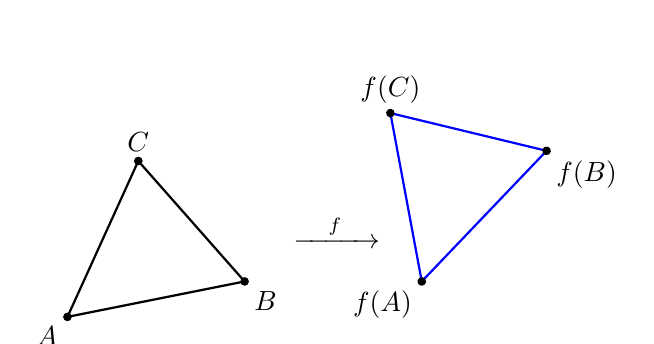
\begin{tikzpicture}[scale=0.9]
  % Original triangle
  \coordinate (A) at (0, 0);
  \coordinate (B) at (2.5, 0.5);
  \coordinate (C) at (1.0, 2.2);
  \draw[thick] (A) -- (B) -- (C) -- cycle;
  \filldraw (A) circle (1.5pt) node[below left] {$A$};
  \filldraw (B) circle (1.5pt) node[below right] {$B$};
  \filldraw (C) circle (1.5pt) node[above] {$C$};

  \node at (3.8, 1.2) {$\xrightarrow{\quad f \quad}$};

  % Rigid moved triangle
  \begin{scope}[shift={(5, 0.5)}, rotate=35]
    \coordinate (Ap) at (0, 0);
    \coordinate (Bp) at (2.5, 0.5);
    \coordinate (Cp) at (1.0, 2.2);
    \draw[thick, blue] (Ap) -- (Bp) -- (Cp) -- cycle;
    \filldraw (Ap) circle (1.5pt) node[below left] {$f(A)$};
    \filldraw (Bp) circle (1.5pt) node[below right] {$f(B)$};
    \filldraw (Cp) circle (1.5pt) node[above] {$f(C)$};
  \end{scope}
\end{tikzpicture}
\caption{剛性運動保持距離與三角形全等}
\label{fig:b4-4-1}
\end{figure}

\begin{proposition}[命題 3]
設 $f$ 為定心剛性運動（$f(O) = O$），則對任意向量 $\mathbf{a}, \mathbf{b}$，恆有
\begin{equation}
f(\mathbf{a}) \cdot f(\mathbf{b}) = \mathbf{a} \cdot \mathbf{b} \label{eq:b4-1-4-2}
\end{equation}
亦卽定心剛性運動保持向量的內積．
\end{proposition}

\begin{proof}[證明]
因 $f$ 保持長度，對任意向量 $\mathbf{a} = \vec{OA}$，有 $|f(\mathbf{a})| = |f(O)f(A)| = |OA| = |\mathbf{a}|$．同理 $|f(\mathbf{b})| = |\mathbf{b}|$，且 $|f(\mathbf{a}) - f(\mathbf{b})| = |f(A)f(B)| = |AB| = |\mathbf{a} - \mathbf{b}|$．

由第三冊向量內積與長度的基本公式：
\[ 2(\mathbf{a} \cdot \mathbf{b}) = |\mathbf{a}|^2 + |\mathbf{b}|^2 - |\mathbf{a} - \mathbf{b}|^2 \]
代入 $f(\mathbf{a})$ 與 $f(\mathbf{b})$：
\begin{align*}
2(f(\mathbf{a}) \cdot f(\mathbf{b})) &= |f(\mathbf{a})|^2 + |f(\mathbf{b})|^2 - |f(\mathbf{a}) - f(\mathbf{b})|^2 \\
&= |\mathbf{a}|^2 + |\mathbf{b}|^2 - |\mathbf{a} - \mathbf{b}|^2 = 2(\mathbf{a} \cdot \mathbf{b})
\end{align*}
故 $f(\mathbf{a}) \cdot f(\mathbf{b}) = \mathbf{a} \cdot \mathbf{b}$．
\end{proof}

\begin{figure}[H]
\centering
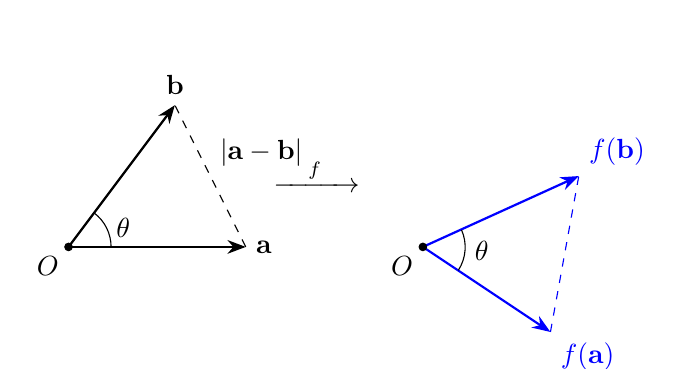
\begin{tikzpicture}[scale=0.9]
  \draw[thick, -Stealth] (0, 0) -- (2.5, 0) node[right] {$\mathbf{a}$};
  \draw[thick, -Stealth] (0, 0) -- (1.5, 2.0) node[above] {$\mathbf{b}$};
  \draw[dashed] (2.5, 0) -- (1.5, 2.0) node[midway, above right] {$|\mathbf{a}-\mathbf{b}|$};
  \draw (0.6, 0) arc (0:53:0.6) node[midway, right] {$\theta$};
  \filldraw (0, 0) circle (1.5pt) node[below left] {$O$};

  \node at (3.5, 1.0) {$\xrightarrow{\quad f \quad}$};

  \begin{scope}[shift={(5, 0)}]
    \draw[thick, -Stealth, blue] (0, 0) -- (1.8, -1.2) node[below right] {$f(\mathbf{a})$};
    \draw[thick, -Stealth, blue] (0, 0) -- (2.2, 1.0) node[above right] {$f(\mathbf{b})$};
    \draw[dashed, blue] (1.8, -1.2) -- (2.2, 1.0);
    \draw (0.5, -0.33) arc (-33:24:0.6) node[midway, right] {$\theta$};
    \filldraw (0, 0) circle (1.5pt) node[below left] {$O$};
  \end{scope}
\end{tikzpicture}
\caption{剛性運動保持內積與夾角}
\label{fig:b4-4-2}
\end{figure}

\begin{proposition}[命題 4]
定心剛性運動保持向量間的夾角（保角性）．
\end{proposition}

\begin{proof}[證明]
夾角餘弦為 $\cos\theta = \dfrac{\mathbf{a} \cdot \mathbf{b}}{|\mathbf{a}| |\mathbf{b}|}$，因分子（內積）與分母（長度）在 $f$ 下皆不變，故 $\cos\theta$ 不變，卽角度不變．
\end{proof}

\begin{proposition}[命題 5]
定心剛性運動必為一線性映射．
\end{proposition}

\begin{proof}[證明]
欲證 $f(\alpha\mathbf{a} + \beta\mathbf{b}) = \alpha f(\mathbf{a}) + \beta f(\mathbf{b})$．令 $\mathbf{w} = f(\alpha\mathbf{a} + \beta\mathbf{b}) - [\alpha f(\mathbf{a}) + \beta f(\mathbf{b})]$，展開其長度平方 $|\mathbf{w}|^2 = \mathbf{w} \cdot \mathbf{w}$，利用命題 3 保持內積之性質逐項展開，可直接算得 $|\mathbf{w}|^2 = 0$，故 $\mathbf{w} = \mathbf{0}$，得證 $f$ 滿足線性條件．
\end{proof}

\subsubsection*{作業 19}
詳細寫出命題 5 證明中計算 $|\mathbf{w}|^2 = 0$ 之全部展開式．

\subsubsection*{乙、正交線性映射}

\begin{definition}[定義]
若線性映射 $f: \mathbf{R}^2 \to \mathbf{R}^2$ 保持向量之長度（亦卽對所有 $\mathbf{x} \in \mathbf{R}^2$ 均有 $|f(\mathbf{x})| = |\mathbf{x}|$），則稱 $f$ 為正交線性映射．
\end{definition}

由命題 5，定心剛性運動與正交線性映射是完全相同的概念！

設 $\{\mathbf{i}_1, \mathbf{i}_2\}$ 為自然基底，令 $\mathbf{e}_1 = f(\mathbf{i}_1), \mathbf{e}_2 = f(\mathbf{i}_2)$．因為 $f$ 保持長度與夾角，且 $\mathbf{i}_1 \perp \mathbf{i}_2, |\mathbf{i}_1| = |\mathbf{i}_2| = 1$，故 $\{\mathbf{e}_1, \mathbf{e}_2\}$ 亦為一正交基底，卽：
\[ |\mathbf{e}_1| = 1, \qquad |\mathbf{e}_2| = 1, \qquad \mathbf{e}_1 \cdot \mathbf{e}_2 = 0 \]
設 $\mathbf{e}_1 = \cos\theta \mathbf{i}_1 + \sin\theta \mathbf{i}_2$，其中 $\theta$ 為 $\mathbf{e}_1$ 的矢角（主矢角 $\theta_0 \in (-\pi, \pi]$）．因 $\mathbf{e}_2 \perp \mathbf{e}_1$ 且 $|\mathbf{e}_2| = 1$，故 $\mathbf{e}_2$ 只有兩種可能位置：
\begin{enumerate}[(i)]
  \item $\mathbf{e}_2$ 之矢角為 $\theta + \dfrac{\pi}{2}$（逆時針 $90^\circ$）．此時
  \[ \mathbf{e}_2 = \cos\left(\theta + \frac{\pi}{2}\right)\mathbf{i}_1 + \sin\left(\theta + \frac{\pi}{2}\right)\mathbf{i}_2 = -\sin\theta\mathbf{i}_1 + \cos\theta\mathbf{i}_2 \]
  \item $\mathbf{e}_2$ 之矢角為 $\theta - \dfrac{\pi}{2}$（順時針 $90^\circ$）．此時
  \[ \mathbf{e}_2 = \cos\left(\theta - \frac{\pi}{2}\right)\mathbf{i}_1 + \sin\left(\theta - \frac{\pi}{2}\right)\mathbf{i}_2 = \sin\theta\mathbf{i}_1 - \cos\theta\mathbf{i}_2 \]
\end{enumerate}

\begin{figure}[H]
\centering
\begin{tikzpicture}[scale=1.1]
  \draw[thick, -Stealth] (-1.5, 0) -- (2.5, 0) node[right] {$\mathbf{i}_1$};
  \draw[thick, -Stealth] (0, -1.5) -- (0, 2.5) node[above] {$\mathbf{i}_2$};
  \draw[gray, dashed] (0, 0) circle (1.5);
  \filldraw (0, 0) circle (1.5pt) node[below left] {$O$};

  % e1
  \draw[very thick, -Stealth, blue] (0, 0) -- (1.3, 0.75) node[above right] {$\mathbf{e}_1$};
  \draw (0.4, 0) arc (0:30:0.4) node[midway, right] {$\theta$};

  % e2 case 1: +90
  \draw[very thick, -Stealth, green!60!black] (0, 0) -- (-0.75, 1.3) node[above left] {$\mathbf{e}_2 = \vec{OE}_2$ (旋轉)};

  % e2 case 2: -90
  \draw[very thick, -Stealth, red] (0, 0) -- (0.75, -1.3) node[below right] {$\mathbf{e}_2' = \vec{OE}_2'$ (鏡射)};
\end{tikzpicture}
\caption{正交基底的兩種方向}
\label{fig:b4-4-3}
\end{figure}

故正交線性映射的自然矩陣表示必為下列兩類之一：
\begin{equation}
\text{第一類：} \quad [f] = \begin{pmatrix} \cos\theta & -\sin\theta \\ \sin\theta & \cos\theta \end{pmatrix} \label{eq:b4-1-4-rot-mat}
\end{equation}
\begin{equation}
\text{第二類：} \quad [f] = \begin{pmatrix} \cos\theta & \sin\theta \\ \sin\theta & -\cos\theta \end{pmatrix} \label{eq:b4-1-4-ref-mat}
\end{equation}

\begin{example}[例 9]
設 $f$ 為一正交線性映射，其將 $\mathbf{i}_1$ 映射為 $\frac{1}{2}\mathbf{i}_1 + \frac{\sqrt{3}}{2}\mathbf{i}_2$，試求 $f$ 的可能自然矩陣表示．
\end{example}

\begin{proof}[解]
由 $\cos\theta = \frac{1}{2}, \sin\theta = \frac{\sqrt{3}}{2}$，知 $\theta = 60^\circ$．
若為第一類，$[f] = \begin{pmatrix} \frac{1}{2} & -\frac{\sqrt{3}}{2} \\ \frac{\sqrt{3}}{2} & \frac{1}{2} \end{pmatrix}$（旋轉 $60^\circ$）．
若為第二類，$[f] = \begin{pmatrix} \frac{1}{2} & \frac{\sqrt{3}}{2} \\ \frac{\sqrt{3}}{2} & -\frac{1}{2} \end{pmatrix}$（鏡射）．
\end{proof}

\subsubsection*{丙、旋轉與鏡射}

\begin{proposition}[命題 6]
當 $f: \mathbf{R}^2 \to \mathbf{R}^2$ 之自然矩陣表示為第一類 \eqref{eq:b4-1-4-rot-mat} 時，$f$ 是平面本身以原點 $O$ 為中心、轉角為 $\theta$ 的旋轉變換．此時 $\det[f] = \cos^2\theta + \sin^2\theta = 1$．
\end{proposition}

\begin{figure}[H]
\centering
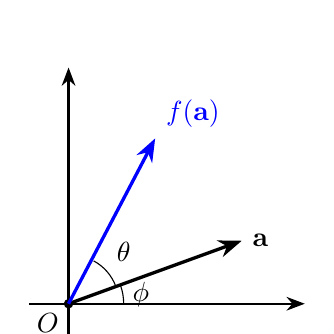
\begin{tikzpicture}[scale=1.0]
  \draw[thick, -Stealth] (-0.5, 0) -- (3, 0);
  \draw[thick, -Stealth] (0, -0.5) -- (0, 3);
  \filldraw (0, 0) circle (1.5pt) node[below left] {$O$};

  \draw[very thick, -Stealth] (0, 0) -- (2.2, 0.8) node[right] {$\mathbf{a}$};
  \draw[very thick, -Stealth, blue] (0, 0) -- (1.1, 2.1) node[above right] {$f(\mathbf{a})$};
  \draw (0.7, 0) arc (0:20:0.7) node[midway, right] {$\phi$};
  \draw (0.6, 0.22) arc (20:62:0.6) node[midway, above right] {$\theta$};
\end{tikzpicture}
\caption{旋轉變換示意圖}
\label{fig:b4-4-4}
\end{figure}

\begin{proposition}[命題 7]
對 $f: \mathbf{R}^2 \to \mathbf{R}^2$，$f$ 為鏡射的充要條件為：存在一正交基底 $\{\mathbf{e}_1, \mathbf{e}_2\}$ 使得任意向量 $\mathbf{a} = \alpha\mathbf{e}_1 + \beta\mathbf{e}_2$，均有
\[ f(\mathbf{a}) = \alpha\mathbf{e}_1 - \beta\mathbf{e}_2 \]
此時稱 $\mathbf{e}_1$ 所在直線 $L$ 為鏡射軸．
\end{proposition}

\begin{figure}[H]
\centering
\begin{tikzpicture}[scale=1.0]
  % Mirror line L
  \draw[thick, dashed] (-1, -0.5) -- (3.5, 1.75) node[right] {$L$ (鏡射軸)};
  \draw[very thick, -Stealth, blue] (0, 0) -- (2, 1) node[above left] {$\mathbf{e}_1$};
  \draw[very thick, -Stealth, blue] (0, 0) -- (-1, 2) node[above left] {$\mathbf{e}_2$};
  \filldraw (0, 0) circle (1.5pt) node[below left] {$O$};

  % Vector a and reflection
  \coordinate (A) at (1.5, 2.5);
  \coordinate (Ap) at (2.5, 0.5);
  \filldraw (A) circle (1.5pt) node[above] {$A (\mathbf{a})$};
  \filldraw (Ap) circle (1.5pt) node[below] {$A' (f(\mathbf{a}))$};
  \draw[thick] (A) -- (Ap);
  \draw[very thick, -Stealth] (0, 0) -- (A);
  \draw[very thick, -Stealth, red] (0, 0) -- (Ap);
\end{tikzpicture}
\caption{鏡射變換幾何圖}
\label{fig:b4-4-5}
\end{figure}

\begin{proposition}[命題 8]
當 $f: \mathbf{R}^2 \to \mathbf{R}^2$ 之自然矩陣表示為第二類 \eqref{eq:b4-1-4-ref-mat} 時，$f$ 是平面中的一個鏡射，而其鏡射軸的傾斜角為 $\dfrac{\theta_0}{2}$，其中 $\theta_0$ 為 $\theta$ 的主矢角．此時 $\det[f] = -\cos^2\theta - \sin^2\theta = -1$．
\end{proposition}

\begin{proposition}[命題 9]
當 $f$ 之自然矩陣表示為第二類時，若取新座標系 $S \equiv (O; \mathbf{e}_1, \mathbf{e}_2)$，其中 $\mathbf{e}_1$ 為鏡射軸，則 $f$ 相關於 $S$ 的矩陣表示為
\[ [f]_S = \begin{pmatrix} 1 & 0 \\ 0 & -1 \end{pmatrix}_S \]
\end{proposition}

\begin{example}[論例 3]
設 $f$ 為轉角 $45^\circ$ 的旋轉，$g$ 為縱軸（$Y$ 軸）的鏡射，則 $g \circ f$ 亦為一鏡射．
\end{example}

\begin{proof}[證明]
因 $[f] = \begin{pmatrix} \cos 45^\circ & -\sin 45^\circ \\ \sin 45^\circ & \cos 45^\circ \end{pmatrix} = \begin{pmatrix} \frac{\sqrt{2}}{2} & -\frac{\sqrt{2}}{2} \\ \frac{\sqrt{2}}{2} & \frac{\sqrt{2}}{2} \end{pmatrix}$，$[g] = \begin{pmatrix} -1 & 0 \\ 0 & 1 \end{pmatrix}$，故
\[ [g \circ f] = [g][f] = \begin{pmatrix} -1 & 0 \\ 0 & 1 \end{pmatrix} \begin{pmatrix} \frac{\sqrt{2}}{2} & -\frac{\sqrt{2}}{2} \\ \frac{\sqrt{2}}{2} & \frac{\sqrt{2}}{2} \end{pmatrix} = \begin{pmatrix} -\frac{\sqrt{2}}{2} & \frac{\sqrt{2}}{2} \\ \frac{\sqrt{2}}{2} & \frac{\sqrt{2}}{2} \end{pmatrix} = \begin{pmatrix} \cos 135^\circ & \sin 135^\circ \\ \sin 135^\circ & -\cos 135^\circ \end{pmatrix} \]
此為第二類正交矩陣，故 $g \circ f$ 為一個對於矢角為 $\frac{135^\circ}{2} = 67.5^\circ$ 直線的鏡射．
\end{proof}

\subsubsection*{作業 20}
若 $f, g$ 為論例 3 中相同的剛性運動，$h$ 表對 $X$ 軸的鏡射：
\begin{enumerate}[(i)]
  \item 試證：$h \circ f$ 仍為一鏡射．
  \item $g \circ h$ 為一旋轉．
  \item 若 $A = (1, 0), B = (2, 1)$，而 $A' = f(A), B' = f(B)$，試證兩者張成平行四邊形面積相等，卽 $\det\begin{pmatrix} a_{11} & a_{21} \\ a_{12} & a_{22} \end{pmatrix} = \det\begin{pmatrix} 1 & 2 \\ 0 & 1 \end{pmatrix} = 1$．
\end{enumerate}

\subsubsection*{丁、總結}

\begin{theorem}[定理 7]
定心剛性運動（卽正交線性映射）不外是平面本身的旋轉或鏡射．若其自然矩陣表示為
\begin{enumerate}[(i)]
  \item $\begin{pmatrix} \cos\theta & -\sin\theta \\ \sin\theta & \cos\theta \end{pmatrix}$，則此映射便是平面本身以原點為心，轉角 $\theta$ 的一個旋轉（$\det = 1$）．
  \item $\begin{pmatrix} \cos\theta & \sin\theta \\ \sin\theta & -\cos\theta \end{pmatrix}$，則此映射便是平面中的一個鏡射，其鏡射軸的矢角為 $\dfrac{\theta}{2}$（$\det = -1$）．
\end{enumerate}
\end{theorem}

\begin{figure}[H]
\centering
\begin{tikzpicture}[scale=0.9]
  \node[draw, rounded corners, fill=blue!10, text width=6cm, align=center] (A) at (0, 2) {\textbf{定心剛性運動（保長保角）}\\$\det A = \pm 1$};
  \node[draw, rounded corners, fill=green!10, text width=4.5cm, align=center] (B) at (-3.5, -0.5) {\textbf{旋轉（Rotation）}\\$\det A = 1$\\保持平面定向（右手系）};
  \node[draw, rounded corners, fill=red!10, text width=4.5cm, align=center] (C) at (3.5, -0.5) {\textbf{鏡射（Reflection）}\\$\det A = -1$\\反轉平面定向（左手系）};
  \draw[thick, -Stealth] (A) -- (B);
  \draw[thick, -Stealth] (A) -- (C);
\end{tikzpicture}
\caption{定心剛性運動之分類體系}
\label{fig:b4-4-6}
\end{figure}

\subsubsection*{作業 21}
轉動 $(-\theta)$ 角之旋轉，其相應的自然矩陣表示為何？特殊地，當轉角為 $-\frac{\pi}{3}$ 時，其自然矩陣表示為何？

\subsubsection*{作業 22}
設 $L$ 為下列直線，求以 $L$ 為鏡射軸的鏡射的自然矩陣表示：
\begin{enumerate}[(i)]
  \item $x - y = 0$
  \item $2x + y = 0$
  \item $y = 0$
\end{enumerate}

\subsubsection*{作業 23}
證明旋轉與鏡射的複合，仍為一鏡射，求其鏡射軸．

\subsubsection*{作業 24}
固定一點 $O$，定義函數 $f_O$ 使得 $\vec{OA'} = -\vec{OA}$．
\begin{enumerate}[(i)]
  \item 試證明 $f_O$ 為一定心剛性運動，卽對 $O$ 點旋轉 $180^\circ$．
  \item 若 $f$ 為一線性映射，且對任意 $A$ 點，$A, O, f(A)$ 三點共線，則 $f$ 為 $\alpha f_O$ 或 $\alpha \mathrm{id}$．
\end{enumerate}

\subsubsection*{作業 25}
\begin{enumerate}[(i)]
  \item 試求定心剛性運動之自然矩陣行列式值 $\det[f]$．
  \item 定心剛性運動為一旋轉的充要條件為 $\det[f] = 1$．
  \item 定心剛性運動為一鏡射的充要條件為 $\det[f] = -1$．
\end{enumerate}

\subsubsection*{作業 26}
\begin{enumerate}[(i)]
  \item $S$ 對 $X$ 軸對稱的充要條件為「$(x, y) \in S \implies (x, -y) \in S$」．
  \item $S$ 對原點對稱的充要條件為何？
\end{enumerate}

\subsubsection*{習題 1-4}
\begin{enumerate}
  \item 
  \begin{enumerate}[(i)]
    \item 試證兩個定心剛性運動相繼作用的結果仍為一定心剛性運動．
    \item 如果 $f: \mathbf{R}^2 \to \mathbf{R}^2$ 為一定心剛性運動，試證有一個唯一的剛性運動 $g$ 使得 $g \circ f = f \circ g = \mathrm{id}$．
    \item 試證 (ii) 中的 $g$ 亦為一定心剛性運動．
  \end{enumerate}

  \item 令 $S_0 \equiv (O; \mathbf{i}_1, \mathbf{i}_2)$ 為 $\mathbf{R}^2$ 的自然座標系．試以 $S_0$ 的座標表示 $\mathbf{u} = 3\mathbf{i}_1 - 4\mathbf{i}_2$ 方向的單位向量，並求以 $\mathbf{u}$ 為鏡射軸之鏡射的自然矩陣表示．

  \item 求下列各組 $\mathbf{u}$ 與 $\mathbf{u}'$ 間的角之正弦及餘弦，並求將 $\mathbf{u}$ 映射為 $\mathbf{u}'$ 的正交線性映射（旋轉與鏡射各一）：
  \begin{enumerate}[a.]
    \item $\mathbf{u} = \frac{\sqrt{3}}{2}\mathbf{i}_1 + \frac{1}{2}\mathbf{i}_2, \mathbf{u}' = \frac{1}{2}\mathbf{i}_1 + \frac{\sqrt{3}}{2}\mathbf{i}_2$
    \item $\mathbf{u} = \mathbf{i}_1 - \sqrt{3}\mathbf{i}_2, \mathbf{u}' = -\mathbf{i}_1 + \sqrt{3}\mathbf{i}_2$
  \end{enumerate}

  \item 求證平面上的映射若保長，則亦保角（提示：利用內積 $2\mathbf{a} \cdot \mathbf{b} = |\mathbf{a} + \mathbf{b}|^2 - |\mathbf{a}|^2 - |\mathbf{b}|^2$）．

  \item 證明任一剛性運動，實際上只是一個定心剛性運動與一個平移相繼作用的結果．
\end{enumerate}
% =========================================================================
% § I-5 正交座標變換
% =========================================================================
\subsection{正交座標變換}
\label{sec:b4-1-5}

如果平面上有兩正交座標系，已知點 $P$ 相關於其中一個座標系的座標，欲求 $P$ 對另一座標系的座標．當然這樣的問題只是第 2 節所申論的一般座標變換之特殊情形．但我們已仔細討論並分類過正交座標系本身之間的線性映射，現在就利用它來直接寫出正交座標變換的形式：

我們先考慮同原點的正交座標變換：

我們不妨把兩正交座標系，取其一為自然座標系 $S_0 \equiv (O; \mathbf{i}_1, \mathbf{i}_2)$，另一正交座標系則記為 $S \equiv (O; \mathbf{e}_1, \mathbf{e}_2)$，$S_0$ 看成舊座標系，$S$ 看成新座標系．已求知（定理 7）：
\begin{equation}
\begin{cases}
\mathbf{e}_1 = \cos\theta\mathbf{i}_1 + \sin\theta\mathbf{i}_2 \\
\mathbf{e}_2 = -\sin\theta\mathbf{i}_1 + \cos\theta\mathbf{i}_2
\end{cases} \quad \text{或} \quad
\begin{cases}
\mathbf{e}_1 = \cos\theta\mathbf{i}_1 + \sin\theta\mathbf{i}_2 \\
\mathbf{e}_2 = \sin\theta\mathbf{i}_1 - \cos\theta\mathbf{i}_2
\end{cases} \label{eq:b4-1-5-1}
\end{equation}
前者代表座標系間的旋轉，後者則代表鏡射．

其所相應的座標變換（由 § I-3 命題 2）按序應為：
\begin{equation}
\begin{cases}
x_1 = \cos\theta x_1' - \sin\theta x_2' \\
x_2 = \sin\theta x_1' + \cos\theta x_2'
\end{cases} \quad \text{或} \quad
\begin{cases}
x_1 = \cos\theta x_1' + \sin\theta x_2' \\
x_2 = \sin\theta x_1' - \cos\theta x_2'
\end{cases} \label{eq:b4-1-5-2}
\end{equation}

\begin{figure}[H]
\centering
\begin{tikzpicture}[scale=1.15]
  \def\ang{22}
  \coordinate (O) at (0, 0);
  % Old axes S0
  \draw[thick, -Stealth] (-1, 0) -- (4.2, 0) node[right] {$x_1$ ($\mathbf{i}_1$)};
  \draw[thick, -Stealth] (0, -0.8) -- (0, 3.8) node[above] {$x_2$ ($\mathbf{i}_2$)};
  \filldraw (O) circle (1.5pt) node[below left] {$O$};

  % Rotated axes S
  \coordinate (E1) at (22:1);
  \coordinate (E2) at (112:1);
  \draw[very thick, -Stealth, blue] (O) -- ($3.8*(E1)$) node[right] {$x_1'$ ($\mathbf{e}_1$)};
  \draw[very thick, -Stealth, blue] (O) -- ($3.5*(E2)$) node[above left] {$x_2'$ ($\mathbf{e}_2$)};
  \draw (0.8, 0) arc (0:22:0.8) node[midway, right=1pt] {\small $\theta$};

  % Point P
  \coordinate (P) at (2.4, 2.4);
  \filldraw (P) circle (2pt) node[above right] {$P(x_1, x_2) = (x_1', x_2')_S$};

  % Projections onto old axes S0
  \draw[densely dashed, gray] (2.4, 0) node[below] {\footnotesize $x_1$} -- (P) -- (0, 2.4) node[left] {\footnotesize $x_2$};

  % Projections onto rotated axes S
  % x1' = 2.4*(cos 22 + sin 22) = 3.125
  % x2' = 2.4*(-sin 22 + cos 22) = 1.325
  \coordinate (Px1p) at ($3.125*(E1)$);
  \coordinate (Px2p) at ($1.325*(E2)$);
  \draw[densely dashed, blue!70!black] (Px1p) node[below right] {\footnotesize $x_1'$} -- (P) -- (Px2p) node[above left] {\footnotesize $x_2'$};
\end{tikzpicture}
\caption{正交座標變換（轉軸）}
\label{fig:b4-5-1}
\end{figure}

但 \eqref{eq:b4-1-5-2} 給的是從新座標求舊座標的式子，實際上的需要常反過來．卽：已知舊座標，要求新座標，此時須分別解 \eqref{eq:b4-1-5-2}，得：
\begin{equation}
\begin{cases}
x_1' = \cos\theta x_1 + \sin\theta x_2 \\
x_2' = -\sin\theta x_1 + \cos\theta x_2
\end{cases} \quad \text{或} \quad
\begin{cases}
x_1' = \cos\theta x_1 + \sin\theta x_2 \\
x_2' = \sin\theta x_1 - \cos\theta x_2
\end{cases} \label{eq:b4-1-5-3}
\end{equation}
前者為旋轉，後者為鏡射的情形．

\begin{example}[例 10]
設 $S \equiv (O; \mathbf{e}_1, \mathbf{e}_2)$ 為一正交座標系，其中
\begin{align*}
\mathbf{e}_1 &= \cos 60^\circ \mathbf{i}_1 + \sin 60^\circ \mathbf{i}_2 \\
\mathbf{e}_2 &= -\sin 60^\circ \mathbf{i}_1 + \cos 60^\circ \mathbf{i}_2
\end{align*}
且 $A = (-2, 1), B = (0, 3)$，求 $A, B$ 的 $S$---座標．
\end{example}

\begin{proof}[解]
由 \eqref{eq:b4-1-5-3} 式
\begin{align*}
A &= \left(-2\cos 60^\circ + \sin 60^\circ, \; (-2)(-\sin 60^\circ) + \cos 60^\circ\right)_S \\
&= \left(-2 \times \frac{1}{2} + \frac{\sqrt{3}}{2}, \; (-2) \times \left(-\frac{\sqrt{3}}{2}\right) + \frac{1}{2}\right)_S = \left(\frac{\sqrt{3}}{2} - 1, \; \sqrt{3} + \frac{1}{2}\right)_S \\
B &= \left(0 \times \cos 60^\circ + 3 \times \sin 60^\circ, \; 0 \times (-\sin 60^\circ) + 3 \times \cos 60^\circ\right)_S = \left(\frac{3\sqrt{3}}{2}, \; \frac{3}{2}\right)_S
\end{align*}
\end{proof}

\subsubsection*{作業 27}
設 $D$ 表座標變換式所相應的矩陣之行列式值〔卽 § I-2 \eqref{eq:b4-1-2-5} 式提出的 $\Delta = a_{11}a_{22} - a_{12}a_{21}$〕，試驗證下列三事：
\begin{enumerate}[(i)]
  \item 正交的座標變換的 $D = \pm 1$．
  \item 當 $D = 1$ 時，卽為旋轉所對應的座標變換．
  \item 當 $D = -1$ 時，卽為鏡射所對應的座標變換．
\end{enumerate}

\subsubsection*{作業 28}
比較 \eqref{eq:b4-1-5-1} 式和 \eqref{eq:b4-1-5-2} 式，其間甚少差別，（代表鏡射的座標變換則完全相同），試和本章第二節中的 (4)，(5) 式相較，原因何在？

\begin{example}[例 11]
設 $S \equiv (O; \mathbf{e}_1, \mathbf{e}_2)$ 為一正交座標系，
\begin{align*}
\mathbf{e}_1 &= \cos\theta\mathbf{i}_1 - \sin\theta\mathbf{i}_2 \\
\mathbf{e}_2 &= \sin\theta\mathbf{i}_1 + \cos\theta\mathbf{i}_2
\end{align*}
若 $A = (\alpha, \beta)_S$，則 $|\vec{OA}| = \sqrt{\alpha^2 + \beta^2}$．
\end{example}

\begin{proof}[證明]
設 $A = (x_1, x_2)$ 則 $x_1 = (\cos\theta)\alpha - (\sin\theta)\beta, x_2 = (\sin\theta)\alpha + (\cos\theta)\beta$，故
\[ |\vec{OA}| = \sqrt{x_1^2 + x_2^2} = \sqrt{\alpha^2 + \beta^2} \]
\end{proof}

\subsubsection*{作業 29}
\begin{enumerate}[(i)]
  \item 在上例若 $\mathbf{e}_1 = \cos\theta\mathbf{i}_1 + \sin\theta\mathbf{i}_2, \mathbf{e}_2 = \sin\theta\mathbf{i}_1 - \cos\theta\mathbf{i}_2$，則亦有 $|\vec{OA}| = \sqrt{\alpha^2 + \beta^2}$．
  \item 若 $S \equiv (O; \mathbf{e}_1, \mathbf{e}_2)$ 為一原點不動的正交座標變換，則對任一點 $A = (\alpha, \beta)_S$ 均有 $|\vec{OA}| = \sqrt{\alpha^2 + \beta^2}$．
  \item 在 (ii) 中 $A, B$ 為任意二點，$A = (x_1, x_2)_S, B = (y_1, y_2)_S$，則 $\vec{OA} \cdot \vec{OB} = x_1 y_1 + x_2 y_2$．
\end{enumerate}

若兩正交座標系 $S_0 \equiv (O; \mathbf{i}_1, \mathbf{i}_2)$ 與 $S \equiv (O'; \mathbf{e}_1, \mathbf{e}_2)$ 的原點不一定相同，則須分兩層討論：
\begin{enumerate}[(1)]
  \item 取 $S' \equiv (O'; \mathbf{i}_1, \mathbf{i}_2)$，因與 $S$ 間的變換是旋轉或鏡射，由 \eqref{eq:b4-1-5-2}
  \begin{equation}
  \begin{cases} x_1' = \cos\theta x_1'' - \sin\theta x_2'' \\ x_2' = \sin\theta x_1'' + \cos\theta x_2'' \end{cases} \quad \text{或} \quad
  \begin{cases} x_1' = \cos\theta x_1'' + \sin\theta x_2'' \\ x_2' = \sin\theta x_1'' - \cos\theta x_2'' \end{cases} \label{eq:b4-1-5-4}
  \end{equation}
  \item 然後因 $S_0 \equiv (O; \mathbf{i}_1, \mathbf{i}_2)$ 與 $S' \equiv (O'; \mathbf{i}_1, \mathbf{i}_2)$ 間只差一平移，設 $\vec{OO'} = b_1\mathbf{i}_1 + b_2\mathbf{i}_2$，則
  \begin{equation}
  \begin{cases} x_1 = x_1' + b_1 \\ x_2 = x_2' + b_2 \end{cases} \label{eq:b4-1-5-5}
  \end{equation}
\end{enumerate}
故將 \eqref{eq:b4-1-5-4} 代入 \eqref{eq:b4-1-5-5} 得自然座標與 $S$ 座標的關係為：
\begin{equation}
\begin{cases}
x_1 = \cos\theta x_1'' - \sin\theta x_2'' + b_1 \\
x_2 = \sin\theta x_1'' + \cos\theta x_2'' + b_2
\end{cases} \quad \text{或} \quad
\begin{cases}
x_1 = \cos\theta x_1'' + \sin\theta x_2'' + b_1 \\
x_2 = \sin\theta x_1'' - \cos\theta x_2'' + b_2
\end{cases} \label{eq:b4-1-5-6}
\end{equation}

總結一下得：

\begin{theorem}[定理 8]
對平面上兩正交座標系 $S_0 \equiv (O; \mathbf{i}_1, \mathbf{i}_2), S \equiv (O'; \mathbf{e}_1, \mathbf{e}_2)$ 的座標變換稱為剛性座標變換，此時兩座標系之關係為：
\begin{equation}
\begin{cases}
\mathbf{e}_1 = \cos\theta\mathbf{i}_1 + \sin\theta\mathbf{i}_2 \\
\mathbf{e}_2 = -\sin\theta\mathbf{i}_1 + \cos\theta\mathbf{i}_2
\end{cases} \quad \text{或} \quad
\begin{cases}
\mathbf{e}_1 = \cos\theta\mathbf{i}_1 + \sin\theta\mathbf{i}_2 \\
\mathbf{e}_2 = \sin\theta\mathbf{i}_1 - \cos\theta\mathbf{i}_2
\end{cases} \label{eq:b4-1-5-thm8-7}
\end{equation}
（前者為旋轉，後者為鏡射），且 $\vec{OO'} = b_1\mathbf{i}_1 + b_2\mathbf{i}_2$．

則其變換式按序為
\begin{equation}
\begin{cases}
x_1 = \cos\theta x_1' - \sin\theta x_2' + b_1 \\
x_2 = \sin\theta x_1' + \cos\theta x_2' + b_2
\end{cases} \quad \text{或} \quad
\begin{cases}
x_1 = \cos\theta x_1' + \sin\theta x_2' + b_1 \\
x_2 = \sin\theta x_1' - \cos\theta x_2' + b_2
\end{cases} \label{eq:b4-1-5-thm8-6}
\end{equation}
其中 $(x_1, x_2), (x_1', x_2')_S$ 分別為平面上點相關於 $S_0$ 與 $S$ 的座標．

特殊地，當 $O = O'$，此時兩種座標間的變換稱同原點剛性座標變換或正交座標變換，兩組基底間的關係仍可由 \eqref{eq:b4-1-5-thm8-7} 式給定．其座標變換式按序為
\[ \begin{cases} x_1 = \cos\theta x_1' - \sin\theta x_2' \\ x_2 = \sin\theta x_1' + \cos\theta x_2' \end{cases} \quad \text{或} \quad \begin{cases} x_1 = \cos\theta x_1' + \sin\theta x_2' \\ x_2 = \sin\theta x_1' - \cos\theta x_2' \end{cases} \]
且易解得
\[ \begin{cases} x_1' = \cos\theta x_1 + \sin\theta x_2 \\ x_2' = -\sin\theta x_1 + \cos\theta x_2 \end{cases} \quad \text{或} \quad \begin{cases} x_1' = \cos\theta x_1 + \sin\theta x_2 \\ x_2' = \sin\theta x_1 - \cos\theta x_2 \end{cases} \]
\end{theorem}

\begin{example}[例 12]
設 $S \equiv (O'; \mathbf{e}_1, \mathbf{e}_2)$ 由一剛性座標變換而得，$\vec{OO'} = \mathbf{i}_1 - \mathbf{i}_2$，$\mathbf{e}_1 = \frac{\sqrt{2}}{2}\mathbf{i}_1 + \frac{\sqrt{2}}{2}\mathbf{i}_2, \mathbf{e}_2 = \frac{\sqrt{2}}{2}\mathbf{i}_1 - \frac{\sqrt{2}}{2}\mathbf{i}_2$．已知 $A = (3, 5), B = (-2, 0)$，求 $A$ 及 $B$ 的 $S$ 座標．
\end{example}

\begin{proof}[解]
由係數比較得知 $S$ 為鏡射的情形．先計算 $A$ 點，$x_1 = 3, x_2 = 5$，代入公式解得 $x_1' = 4\sqrt{2}, x_2' = -2\sqrt{2}$，故 $A = (4\sqrt{2}, -2\sqrt{2})_S$．

同理計算點 $B$：$x_1 = -2, x_2 = 0$，得 $B = (-2\sqrt{2}, -\sqrt{2})_S$．
\end{proof}

\subsubsection*{作業 30}
設 $S$ 為上例中的座標系：
\begin{enumerate}[(i)]
  \item $A, B, C$ 之自然座標分別為 $(5, 1), (0, 3), (-2, -2)$ 求其 $S$---座標．
  \item 若 $A, B, C$ 之 $S$---座標為 $(0, 2)_S, (1, 1)_S, (-1, 3)_S$，求其自然座標．
\end{enumerate}

\subsubsection*{習題 1-5}
\begin{enumerate}
  \item 一個圓形木板半徑為 $1$ 公尺在平面上沿一直線順時鐘方向滾動，在原點取一自然座標系 $S_0 \equiv (O; \mathbf{i}_1, \mathbf{i}_2)$．另於木板上在圓心 $O'$ 上取一正交座標系 $S \equiv (O'; \mathbf{i}_1', \mathbf{i}_2')$ 固定于木板上，設木板轉動之角速度為每秒鐘一弧度．
  \begin{enumerate}[(i)]
    \item 問在轉動開始後在第 $6$ 秒鐘時，$S$ 與 $S_0$ 間的關係如何？
    \item 在起始時，木板上的點 $P$ 為 $(\frac{1}{2}, \frac{1}{2})_S$，到轉動開始後第 $10$ 秒時，點 $P$ 相關于 $S_0$ 的座標如何？
  \end{enumerate}

  \item 上題中如該木板的圓心固定在點 $O$ 順時鐘方向轉動，則答案如何？
\end{enumerate}

\vspace{1.5em}
\noindent\textbf{〔章末附註〕}\phantomsection\label{note:b4-ch1-p57-appendix-note}

一般說來，一個映射（或稱函數）就是將一個集合 $S$ 中的元素（照）射到另一集合 $T$ 中的元素的函數．$S$ 仍稱為定義域；$T$ 為值域，寫成 $f: S \to T$．若 $s \in S$，稱 $f(s) \in T$ 為 $s$（經映射 $f$）的像點．而若 $A \subset S$，稱 $f(A)$ 為集合 $A$（經映射 $f$）的映像（Image）（或像集），記作
\[ f(A) = \{f(x) \mid x \in A\} \]

對於 $S$ 集合中不同的元素 $s_1, s_2$，若它在 $T$ 中的像點 $f(s_1)$ 與 $f(s_2)$ 也不相同，卽
\[ s_1, s_2 \in S, \; s_1 \neq s_2 \implies f(s_1) \neq f(s_2) \]
我們就說：$f$ 是嵌射的（injective）映射，或 $f$ 是嵌射（injection）（又稱單射，或一一映至）．

若對於 $T$ 中任意 $t$，存在至少一個 $s \in S$，使得 $f(s) = t$，我們就說：$f$ 是 $S$ 到 $T$ 的蓋射（surjection），或 $f$ 為蓋射的（surjective）映射（又稱全射）．

如果 $f$ 是蓋射的，又是嵌射的，就叫對射的（bijective），或 $f$ 稱為一個對射（bijection），（亦卽一一映成）．

（若 $f$ 不是蓋射的，對 $t \in T$，不必存在 $s \in S$，使得 $f(s) = t$）但是若對 $t \in T$，存在 $s \in S$ 使得 $f(s) = t$，則任意如此 $s$，均稱為 $t$ 的一個像原，我們用 $s \in f^{-1}(t)$ 表示，卽若 $B \subset T$，$S$ 的子集 $f^{-1}(B) = \{s \mid f(s) \in B\}$ 稱為 $B$ 的像原（Preimage）．

給定兩映射 $f: S \to T$ 及 $g: T \to V$，則由 $S$ 到 $V$ 的映射，使得任意 $S$ 中的元素 $s$ 的像點為：
\[ h(s) = g(f(s)) \]
稱為 $f$ 與 $g$ 的合成或複合映射，記為 $h = g \circ f$．


\end{document}
